\documentclass[11pt]{book}

\usepackage{fullpage}
\usepackage{graphicx}
\usepackage{cite}
\usepackage{times}
\usepackage{url}
\usepackage{hyperref}
\usepackage{setspace}
\usepackage{fancyhdr}
\usepackage{ifthen}
\usepackage{listings}
\usepackage[section]{placeins}
\usepackage{xtab}
\usepackage{booktabs}
\usepackage{float}

\setcounter{topnumber}{2}
\setcounter{bottomnumber}{3}
\setcounter{totalnumber}{4}
\renewcommand{\topfraction}{0.5}
\renewcommand{\bottomfraction}{0.95}
\renewcommand{\textfraction}{0.1}
\renewcommand{\floatpagefraction}{0.7}

\setlength{\abovecaptionskip}{3pt}
\setlength{\belowcaptionskip}{3pt}

\pagestyle{fancy}
\setboolean{@twoside}{false}
\setlength{\headsep}{25pt}
\setlength{\headheight}{14pt}

\begin{document}

\thispagestyle{empty}

\doublespacing

\vspace*{0.5in}

\begin{center}
  \LARGE{\textbf{Reducing Network Latency for Low-cost Beowulf Clusters}}

  \vspace*{0.4in}

  {\large A thesis submitted to the\\[0.20in]
    Division of Research and Advanced Studies\\
    of the University of Cincinnati\\[0.20in]
    in partial fulfillment of the\\
    requirements for the degree of\\[0.20in]
    {\bf MASTER OF SCIENCE}\\[0.20in]
    in the School of Electric and Computing Systems\\
    of the College of Engineering and Applied
    Sciences\\[0.20in]
    July TODO, 2014\\[0.20in]
    by\\[0.20in]
    {\bf Eric Carver}\\
    BSEE, University of
    Cincinnati, 2014\\}
  \vspace{0.5in}
  {\large Thesis Advisor and Committee Chair:  Dr. Philip A. Wilsey}
\end{center}

\clearpage

\setcounter{page}{1}
\pagenumbering{roman}
\clearpage

\chapter*{Abstract}

%% TODO: Write abstract

\chapter*{Acknowledgements}

\tableofcontents \markright{ }
\listoffigures \markright{ }
\listoftables \markright{ }

\clearpage
\pagenumbering{arabic}
\setcounter{page}{1}

\chapter{Introduction}
\label{introduction}

The applications of Beowulf clusters have expanded since Becker et al. created
the first one in 1995 \cite{becker-95}. Although originally intended for
scientific computing, this ``network-of-worstations'' technology has also been
adopted for use in data centers \cite{liu-13}, cloud computing
\cite{trivedi-11}, and research in fine-grained parallel computing
\cite{aad-03}. Because these workstations are self contained and connected
through a network, the bandwidth and latency of their interconnect are
determining factors of a Beowulf cluster's performance \cite{lancaster-10}
\cite{becker-95}. This is particularly true for fine-grained parallelism, where
messages must be passed frequently in order to utilize the processing power of
the cluster.

Even small Beowulf clusters typically cost many thousands of dollars. This
limits their availability to researchers in two ways. First, many academic
institutions cannot afford any type of traditional Beowulf cluster. Second,
those who can afford one must restrict access to the cluster because many
researchers need to use it. This need to administer the cluster as a shared
environment eliminates the possibility of exploring custom hardware and
operating system services targeted to increase cluster performance for
fine-grained parallel applications.

Additionally, once an institution sinks the high cost of a traditional Beowulf
cluster, the institution is naturally reluctant to upgrade the cluster for many
years. This can prevent researchers from accessing new innovations in hardware
and their associated features for many years.

However, the emergence of small form factor symmetric multiprocessing (SMP)
computing platforms has created an opportunity to create a new class of Beowulf
cluster. Driven by the quickly increasing computing demands of small form factor
computers such as cellular telephones, tablet computers, and netbooks, mobile
computing platforms have increased dramatically in computing power in the last
few years. However, there has been little interest in applying these low-cost
processors to solve availability issues in high-performance computing (HPC)
research.

The Samsung Exynos 5410 system-on-a-chip (SoC) is an example of a powerful, yet
low cost SMP platform. Its eight processor cores promise excellent raw computing
performance for those who are able to utilize it.

Currently, the design of these mobile SMP platforms presents some challenges to
those who wish to use them as nodes in a high-performance cluster. In
particular, end-to-end network latency can be orders of magnitude greater than
one would expect to find in a traditional Beowulf cluster. In order to minimize
the impact of this limitation on computing performance, we have embarked on
research into software-based methods of reducing network latency.

\section{\textbf{Research Statement}}

We believe that it is possible to create a Beowulf cluster using small form
factor computers that delivers a performance-for-price ratio comparable to the
ratio of some traditional Beowulf clusters, especially those that are at least a few
years old. In particular, we want to achieve such a ratio for performance in
parallel discrete event simulation (PDES).

The primary obstacle to this objective is the high network latency associated
with many small form factor computers. Therefore, this research will focus on
two methods of reducing that latency at no additional cost: software Remote
Direct Memory Access (RDMA) over Converged Ethernet (RoCE) and polling network
drivers.

\section{\textbf{Thesis Overview}}

The remainder of this thesis is organized as follows.

Chapter \ref{background} provides background information on Parallel Discrete
Event Simulation (PDES), Infiniband\texttrademark, and small form factor
computers, including the ODROID platform used in this research.

Chapter \ref{latency_reduction} presents our strategy for attacking the network
latency problem in our Beowulf cluster. It focuses on two low-cost solutions:
software RDMA over Converged Ethernet (RoCE) and polling network drivers.

Chapter \ref{cluster} describes the hardware and software implementation of the
ODROID-XU cluster constructed as part of these experiments and details the
benchmarks and simulations used to test its performance.

Chapter \ref{results} provides the results of these tests and attempts to relate
the cluster's performance to its cost. The results of a similar set of tests on
a traditional cluster are provided for comparison.

Chapter \ref{conclusions} contextualizes the results of this research and
suggests ways to continue this work.

\newpage
\chapter{Background}
\label{background}

\section{\textbf{Parallel Discrete Event Simulation}}

\section{\textbf{Infiniband and RoCE}}

\href{www.infinibandta.org}{InfiniBand}\texttrademark (IB) was introduced in
1999 to meet the new demand of data-intensive applications in high-end computing
environments \cite{InfiniBandTABase-07}. Its characteristic high bandwidth and
low latency make it a popular interconnect technology for computing solutions
intended for fine-grained parallel simulation. For high-end Beowulf Clusters,
message latency as low as one microsecond is provided through the two-pronged
approach of using InfiniBand networking hardware and the lightweight IB
transport layer. However, the high cost and lack of inter-fabric compatibility
of such hardware have driven the development of solutions based on the
ubiquitous Ethernet link layer \cite{roce-announce}.

Although IB is a full first-order interconnect solution, its transport layer is
particularly attractive to researchers who desire affordable high performance
computing. It specifies four transport types: Reliable Connection (RC), Reliable
Datagram (RD), Unreliable Connection (UC), and Unreliable Datagram (UD)
\cite{InfiniBandTABase-07}. All four types support channel messaging semantics,
wherein messages are passed using send and receive calls
\cite{InfiniBandTABase-07}. The RC and UC types support memory semantics, also
known as Remote Direct Memory Access (RDMA). This approach allows an initiator
computing node to access the memory of a remote process directly, without any
significant effort on the part of the remote node \cite{sur-11}.

RDMA over Converged Ethernet (RoCE), also known as Infiniband over Ethernet
(IBoE), is an attempt to provide the reliable, low-latency InfiniBand transport
services over a converged Ethernet fabric already present in most data centers
\cite{InfiniBandTARoCE-10}, \cite{roce-announce}. This enables properly
configured networks to carry IB traffic without investing in entirely new
physical hardware. Message latency can be under 2 microseconds when used in a
lossless 40 Gigabit Ethernet network \cite{vienne-12}. RoCE has found a niche in
commercial data centers, especially those that support financial operations such
as high frequency trading. Unfortunately, specialized network adaptors are still
required to take advantage of its features. Additionally, these solutions
generally require switches that support Data Center Bridging (DCB)
\cite{InfiniBandTARoCE-10}. This creates an opportunity for a solution that can
work with existing lossy Ethernet networks.

%% TODO: Discuss iWARP

System Fabric Works, Inc., has created a pure software implementation of RoCE
called \href{http://www.systemfabricworks.com/downloads/roce}{rxe}. \verb;rxe;
is a Linux driver that implements the full IB transport over any Ethernet
adaptor \cite{pearson-10}. Message latency can be as low as 10
microseconds on a 10 Gigabit Ethernet controller \cite{pearson-10}. The
\href{http://support.systemfabricworks.com/downloads/rxe/}{most recent relase of
  the driver} is in the from of patches for the mainline Linux kernel. We chose
to port this implementation to the ODROID platform for our studies in low-cost
Beowulf Clusters.


\section{\textbf{ODROID Platform}}

The ODROID series of development boards from Hardkernel Co., Ltd. has made
low-cost mobile hardware available in more traditional computing platforms. In
these studies, we focus on the ODROID-U2 and ODROID-XU boards. The
characteristics of these two platforms are given in the next two sections.

\subsection{\textbf{ODROID-U2}}

\begin{figure}[H]
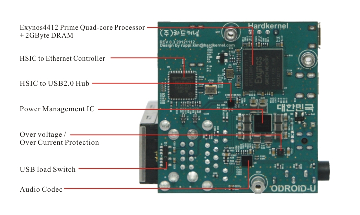
\includegraphics[width=\textwidth]{odroid_u2_top}
\caption{ODROID-U2 circuit board top view\cite{odroid-u2-board-detail}}
\label{odroid-u2-board}
\end{figure}

\begin{figure}[H]
\centering
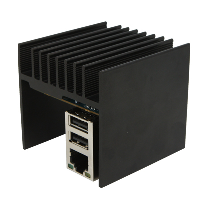
\includegraphics[width=0.5\textwidth]{odroid_u2}
\caption{ODROID-U2 with heatsink \cite{odroid-u2-board-detail}}
\label{odroid-u2}
\end{figure}

The ODROID-U2 board hosts a Samsung Exynos 4412 Prime System on a Chip
(SoC). \textbf{Figure \ref{odroid-u2-board}} shows the board on its own, and
\textbf{Figure \ref{odroid-u2}} shows the board installed in its heatsink. The
board features the following hardware components:

\begin{itemize}
\item Samsung Exynos 4412 Prime
  \begin{itemize}
  \item 4 ARM Cortex-A9 cores clocked at 1.7 GHz
  \item 2 GB LPDDR2 capable of 880 MT/s
  \end{itemize}
\item SMSC USB3503A USB 2.0 hub
\item SMSC LAN9730 USB 2.0 to 100 Mpbs Ethernet controller
\item MAXIM MAX98098 Audio CODEC
\end{itemize}

While the ODROID-U2 features impressive raw processing power for its size and
price, its small of main memory can adversely impact performance for even
moderately sized parallel simulation models. The Exynos SoC 

\subsection{\textbf{ODROID-XU}}

\section{\textbf{Related Work}}

%% ERIC: do we know of any related work?  even publications talking about
%% IBoE/RoCE performance on the x86 platform would be worth reviewing.

Although performance profiling of hardware IB and RoCE is extensive
\cite{subamaroni-09}, \cite{vienne-12}, studies on software RoCE are
rare. Robert J. Lancaster \cite{lancaster-10} experimented with the rxe
driver. He found that \verb;rxe; message latency ranged from 14\% to 81\% lower
than TCP/IP using a Realtek 8168B Gigabit Ethernet adaptor with the r8169
driver.

Trivedi et al. \cite{trivedi-11} experimented with a software implementation of
iWARP for use in cloud computing. They found that end-to-end latencies were
reduced for messages larger than 64 kB thanks the protocol's lightweight RDMA
implementation.

%% Can't really find anything else on softroce

\newpage
\chapter{Methods for Reducing Network Latency}
\label{latency_reduction}

\section{\textbf{Software RoCE}}

Currently, there is only one open-source software RoCE project: the \verb;rxe;
linux driver. System Fabric Works created the driver with at least two goals in
mind: to provide a low-cost gateway to Infiniband software and to function as a
testbed for IB application development \cite{pearson-10}. In both cases, its
lack of network hardware dependence distinguishes it from all other Infiniband
implementations. We hoped to leverage this technology for use in our low-cost
cluster in order to bring its performance closer to the performance of a
traditional x86 cluster.

\begin{figure}[H]
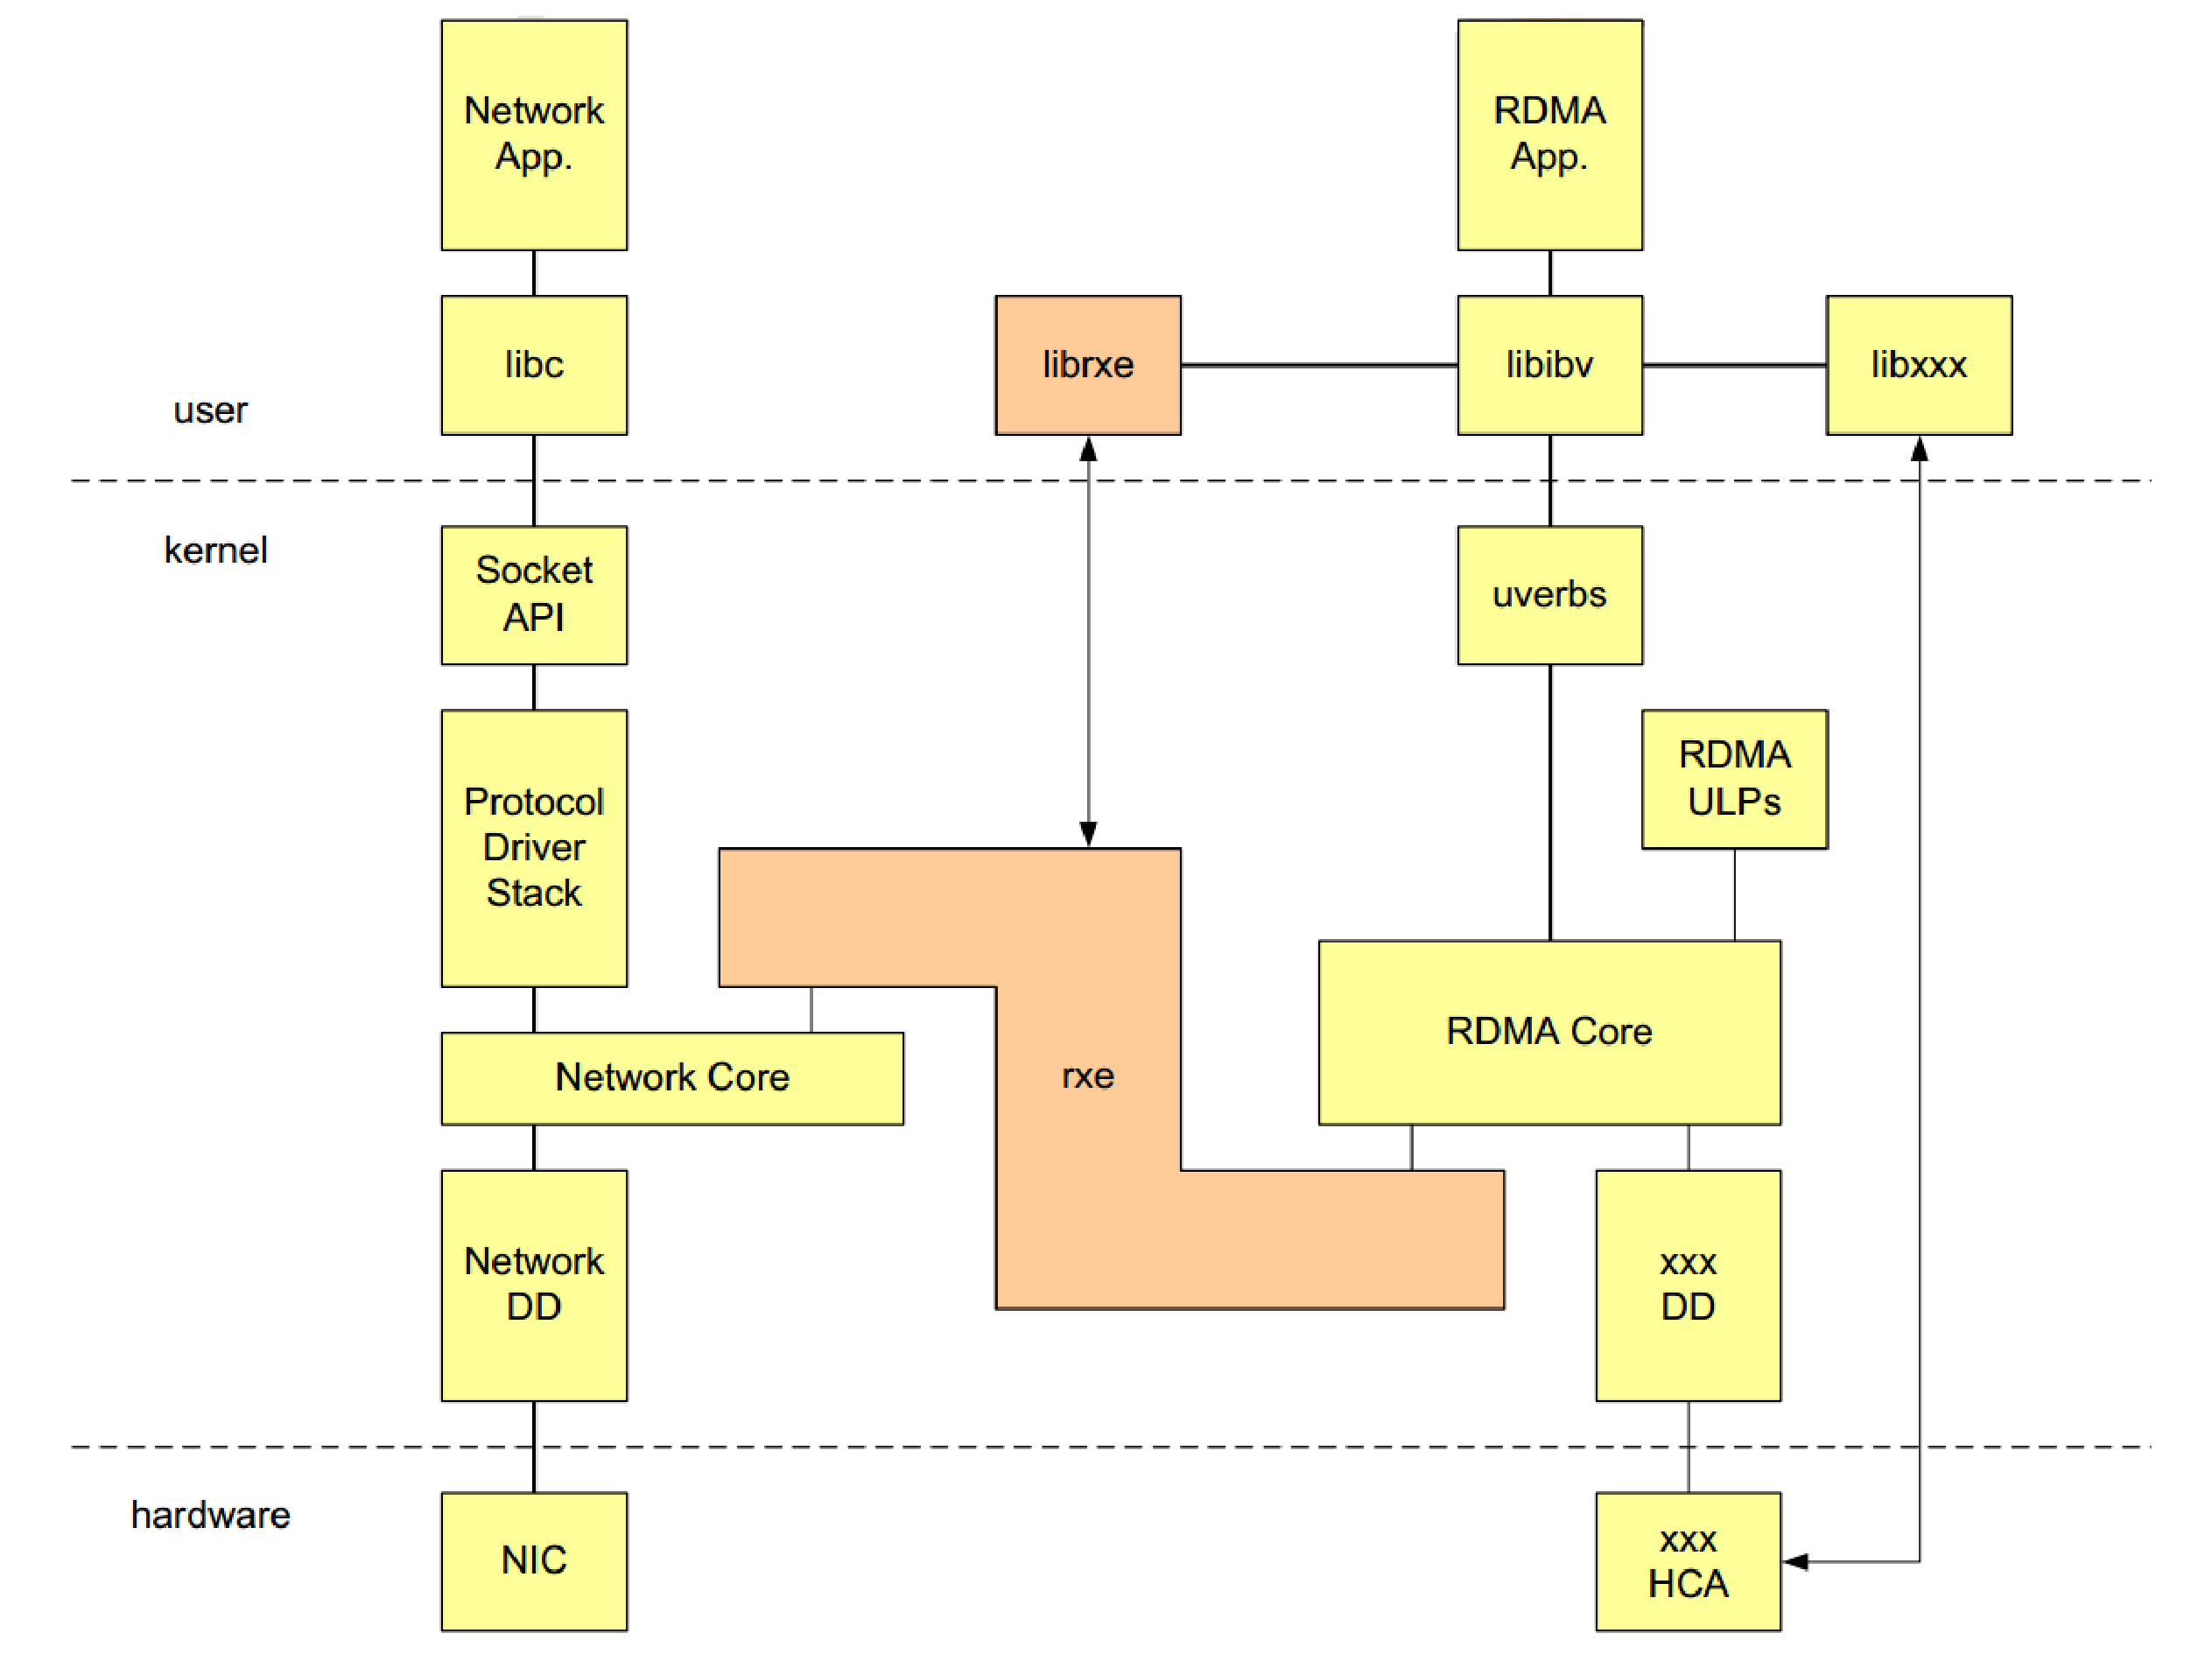
\includegraphics[width=\textwidth]{rxe_linux}
\caption{rxe driver role in a Linux networking environment \cite{pearson-10}}
\label{rxe-linux}
\end{figure}

\textbf{Figure \ref{rxe-linux}} illustrates how the \verb;rxe; driver functions
as a bridge between RDMA software and the Linux networking core.

The \verb;rxe; linux driver is divided into two modules: \verb;rxe; and
\verb;rxe-net; \cite{pearson-10}. \verb;rxe; provides an implementation of the
Infiniband transport compliant with the RoCE specification annex
\cite{InfiniBandTARoCE-10}. \verb;rxe-net; interfaces with the Linux networking
stack to transmit and receive packets earmarked for \verb;rxe;
\cite{pearson-10}. The following two sections detail the design of these
modules.

The \verb;rxe; driver also interfaces with a user-mode library called
librxe. This library provides the common Infiniband\texttrademark verbs
interface so that any compliant IB application can use the \verb;rxe; device
without any modification. This library is essentially a user-mode wrapper for
the functions found in the rxe driver, so its design will not be detailed here.

\subsection{\textbf{rxe}}
\label{rxe}

The \verb;rxe; kernel module contains the portion of the \verb;rxe; driver that
implements layers 4 through 7 of the OSI model. It provides a software
implementation of the Infiniband\texttrademark RoCE transport. As with all IB
verbs applications, memory is preallocated in Memory Regions (MR), and coupled
pairs of send and receive queues called ``queue pairs'' (QPs) are allocated by
the application based on its needs. That is, QPs are configurable at allocation
time in terms of both queue depth and entry length
\cite{InfiniBandTARoCE-10}\cite{InfiniBandTABase-07}. QPs can be resized after
they are created, but such an operation may adversely impact performance
\cite{InfiniBandTARoCE-10}.

\begin{figure}[H]
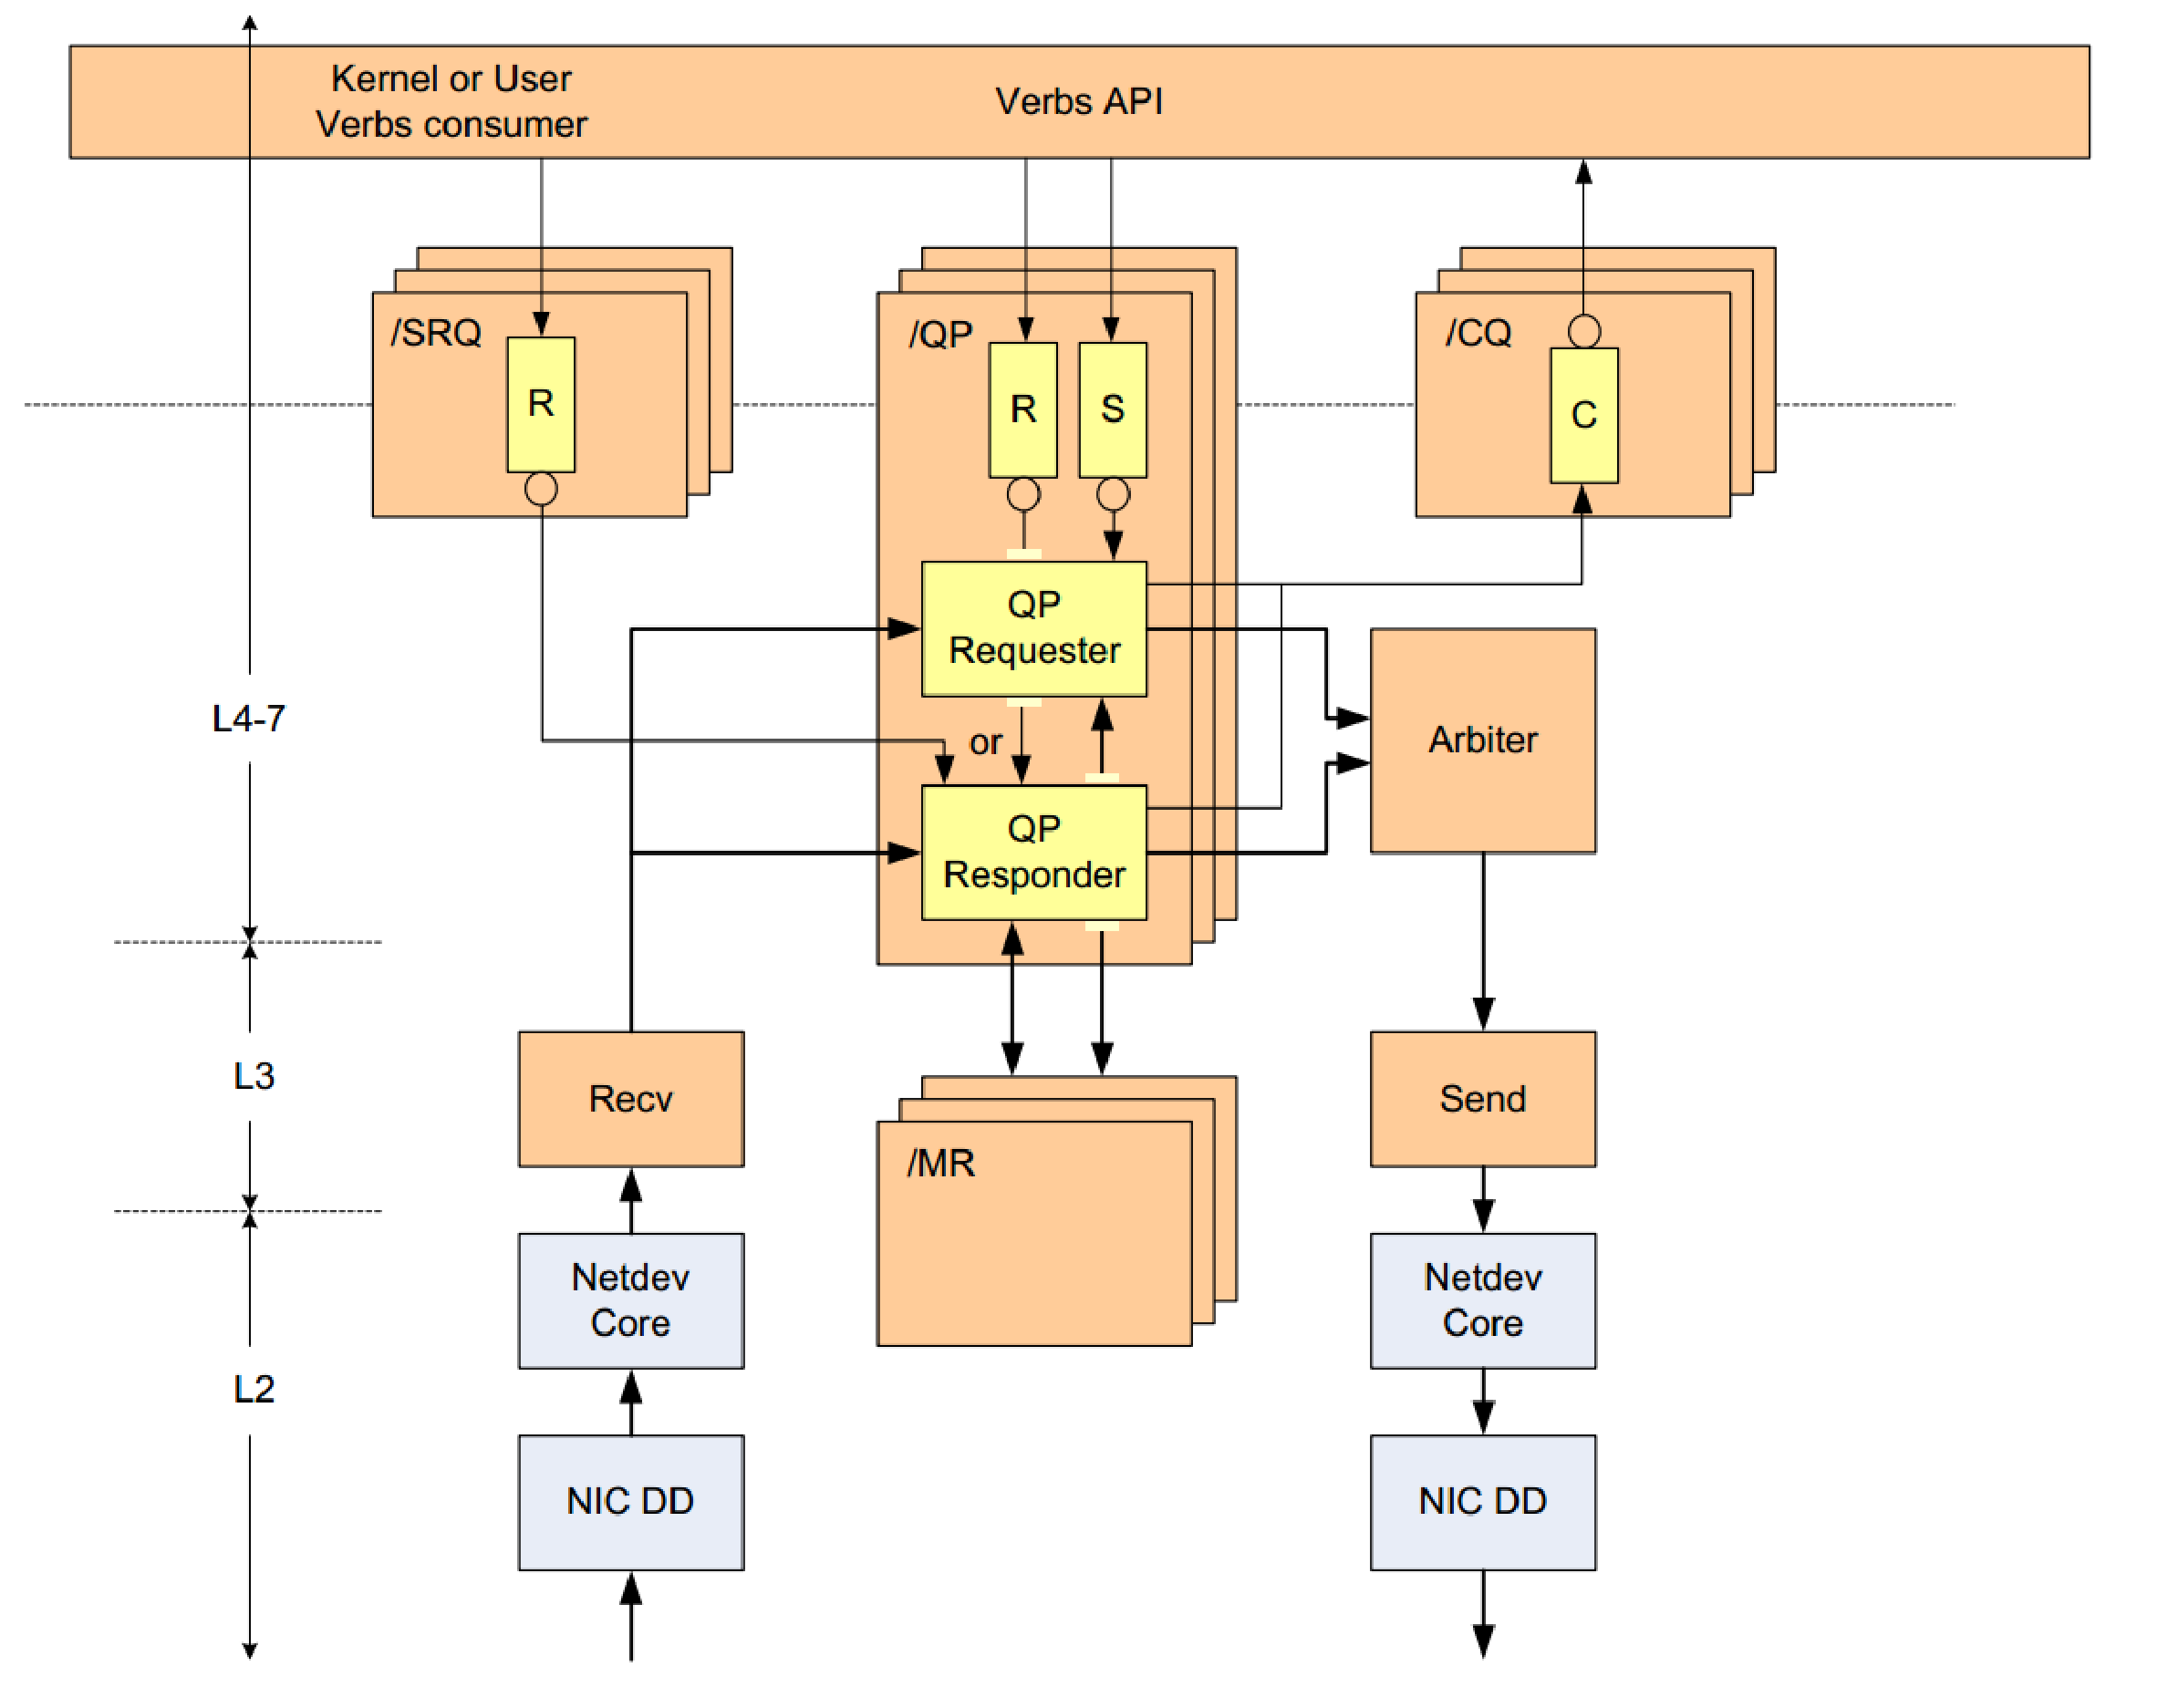
\includegraphics[width=\textwidth]{rxe_overview}
\caption{rxe driver overview \protect\cite{pearson-10}}
\label{rxe-overview}
\end{figure}

\textbf{Figure \ref{rxe-overview}} shows the dataflow among the major partitions
of the rxe driver. When a consumer application intends to send or receive a
message, it must submit a Work Request (WR) via an IB verbs function call. This
function places the WR into a QP allocated for that application. If the
application uses Shared Receive Queue (SRQ) semantics (as OpenMPI does), then
another small wrinkle is added for receive WRs as both the SRQ and the QP
associated with the WR must be resolved. Once the Linux kernel is notified that
a WR has been enqueued, the QP Requester and QP Responder routines work to
complete that request. When a WR has been completed, and entry is placed in a
Completion Queue (CQ) that can be accessed by the verbs application. This
Completion Queue Entry (CQE) contains information that the application needs in
order to consider the WR completed.

\begin{figure}[H]
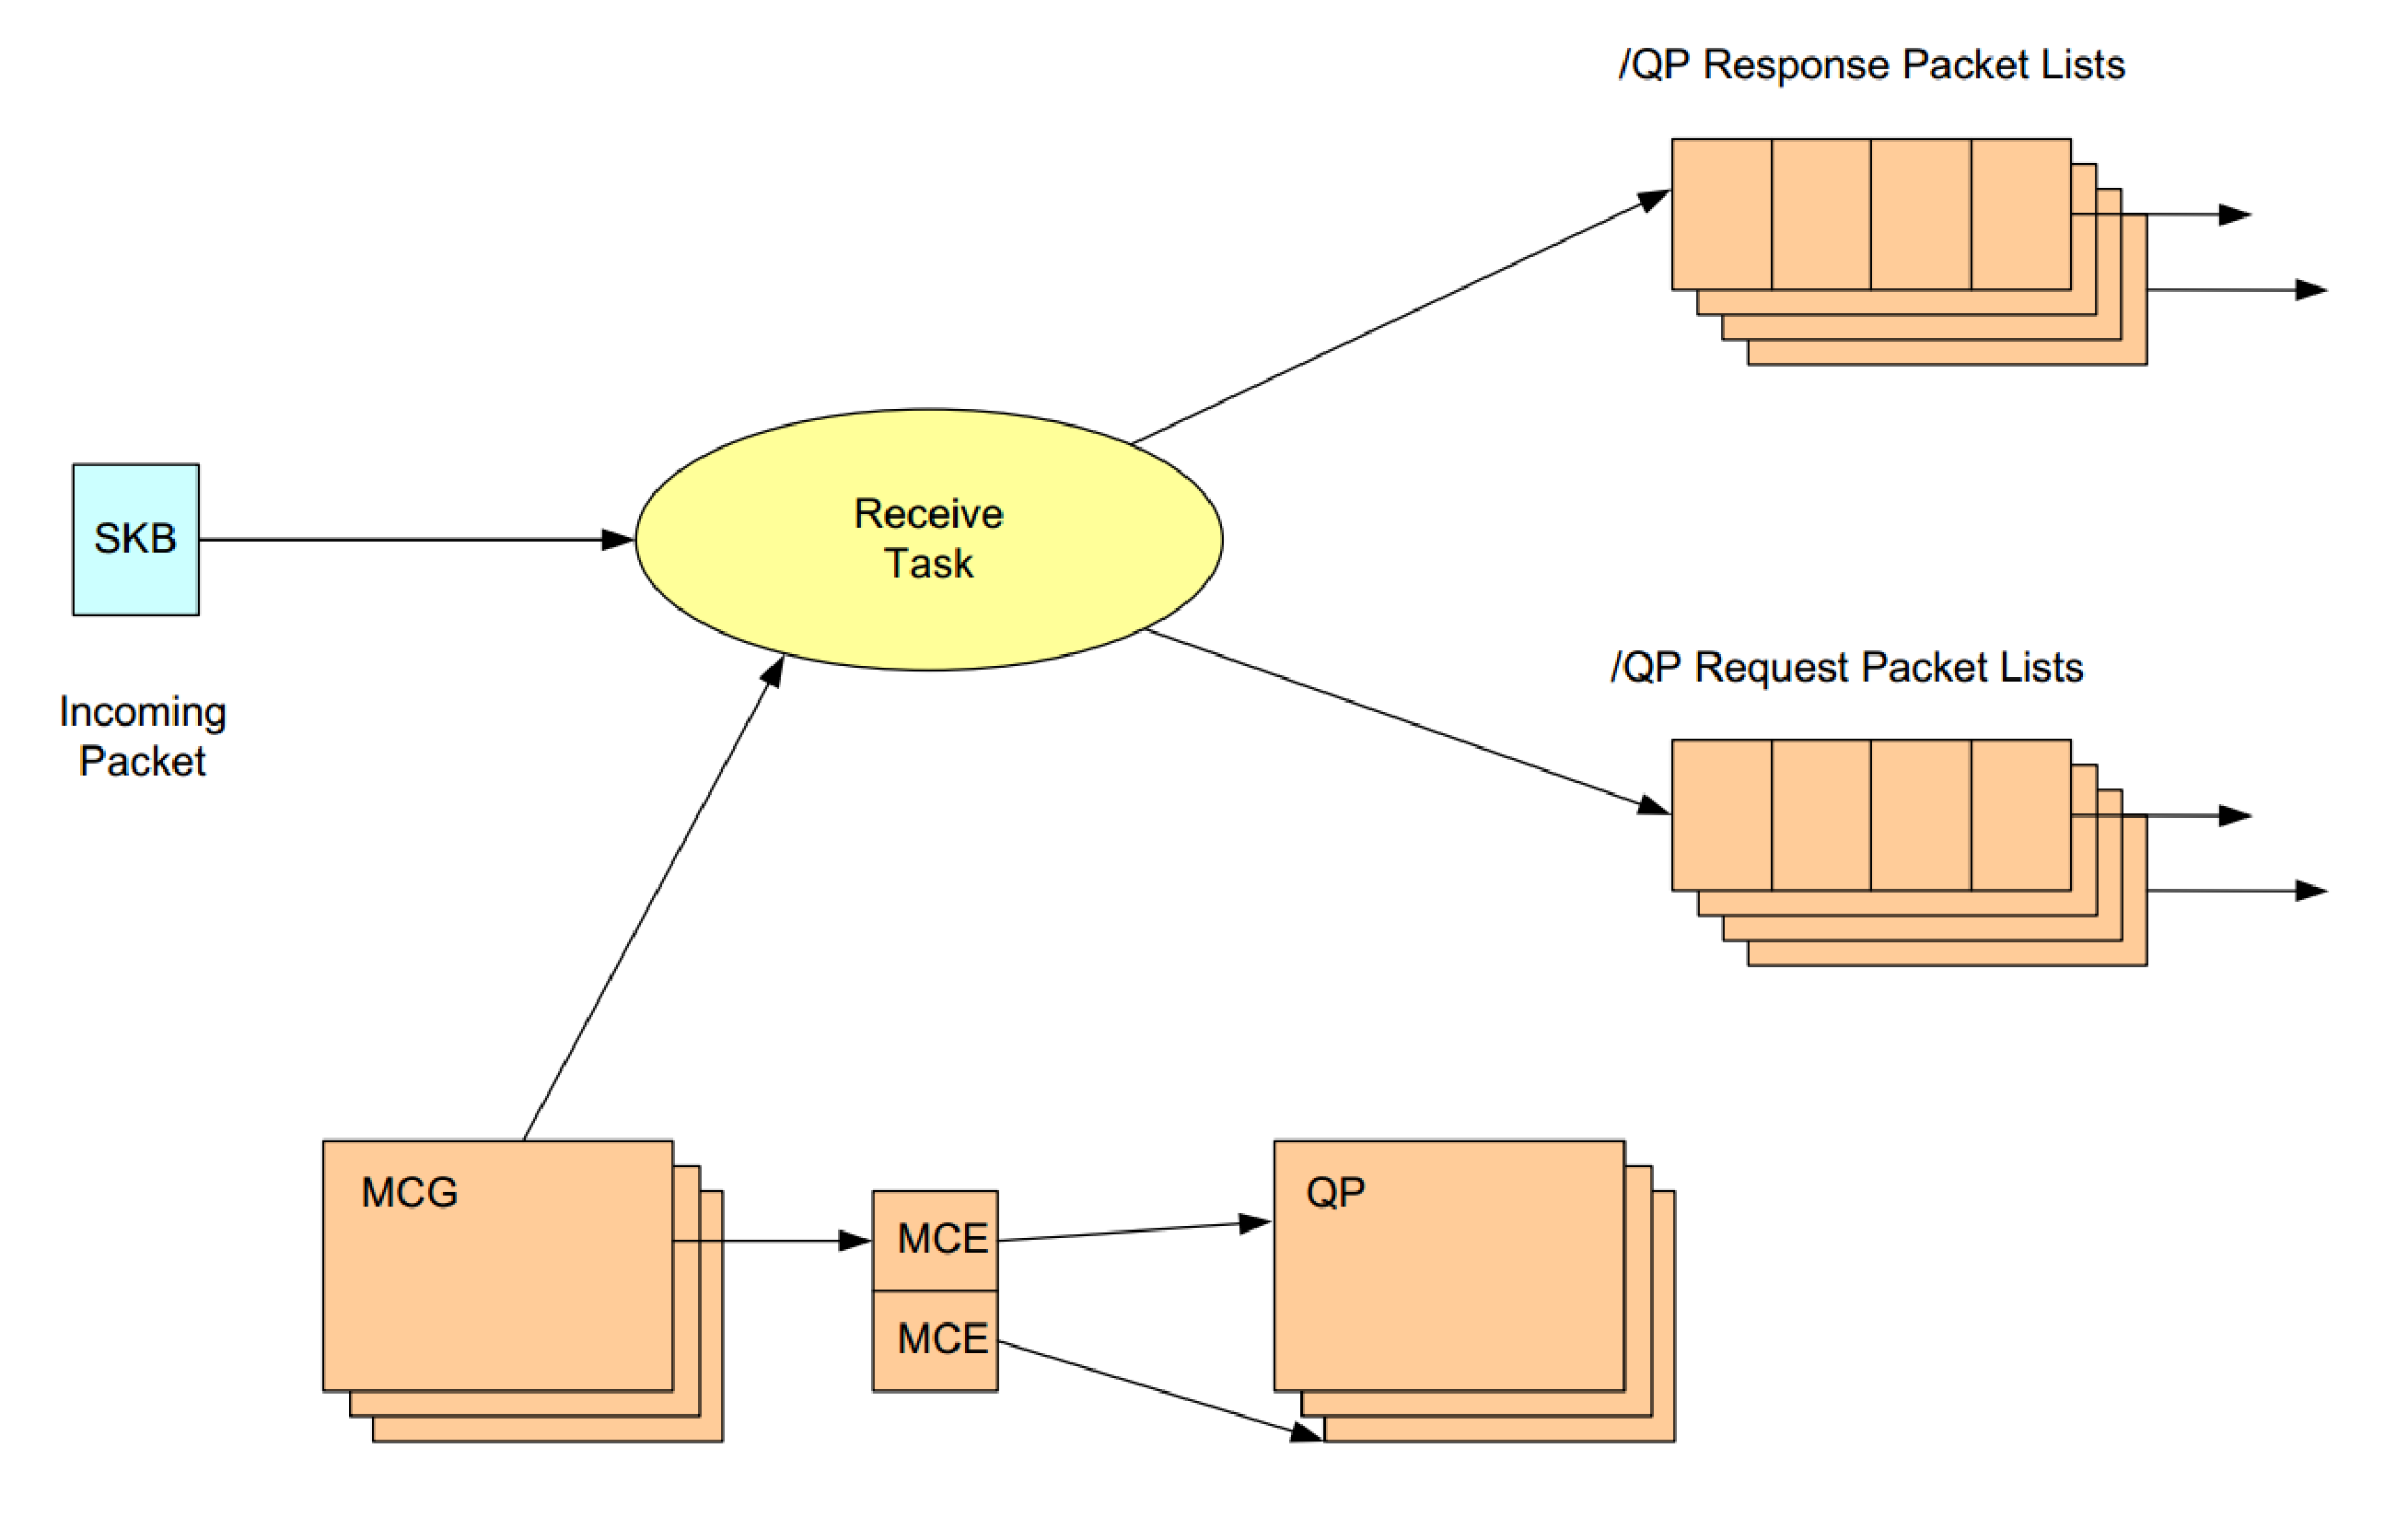
\includegraphics[width=\textwidth]{rxe_recv}
\caption{rxe Receive task \protect\cite{pearson-10}}
\label{rxe-recv}
\end{figure}

The Layer 4 portion of the \verb;rxe; driver's Receive routine is illustrated in
\textbf{Figure \ref{rxe-recv}}. This function receives a socket buffer (SKB)
from \verb;rxe-net; as an input. It inspects the SKB header in order to
determine whether the message is a response packet or a request packet and
places the SKB into a corresponding packet list in the receive queue.

\begin{figure}[H]
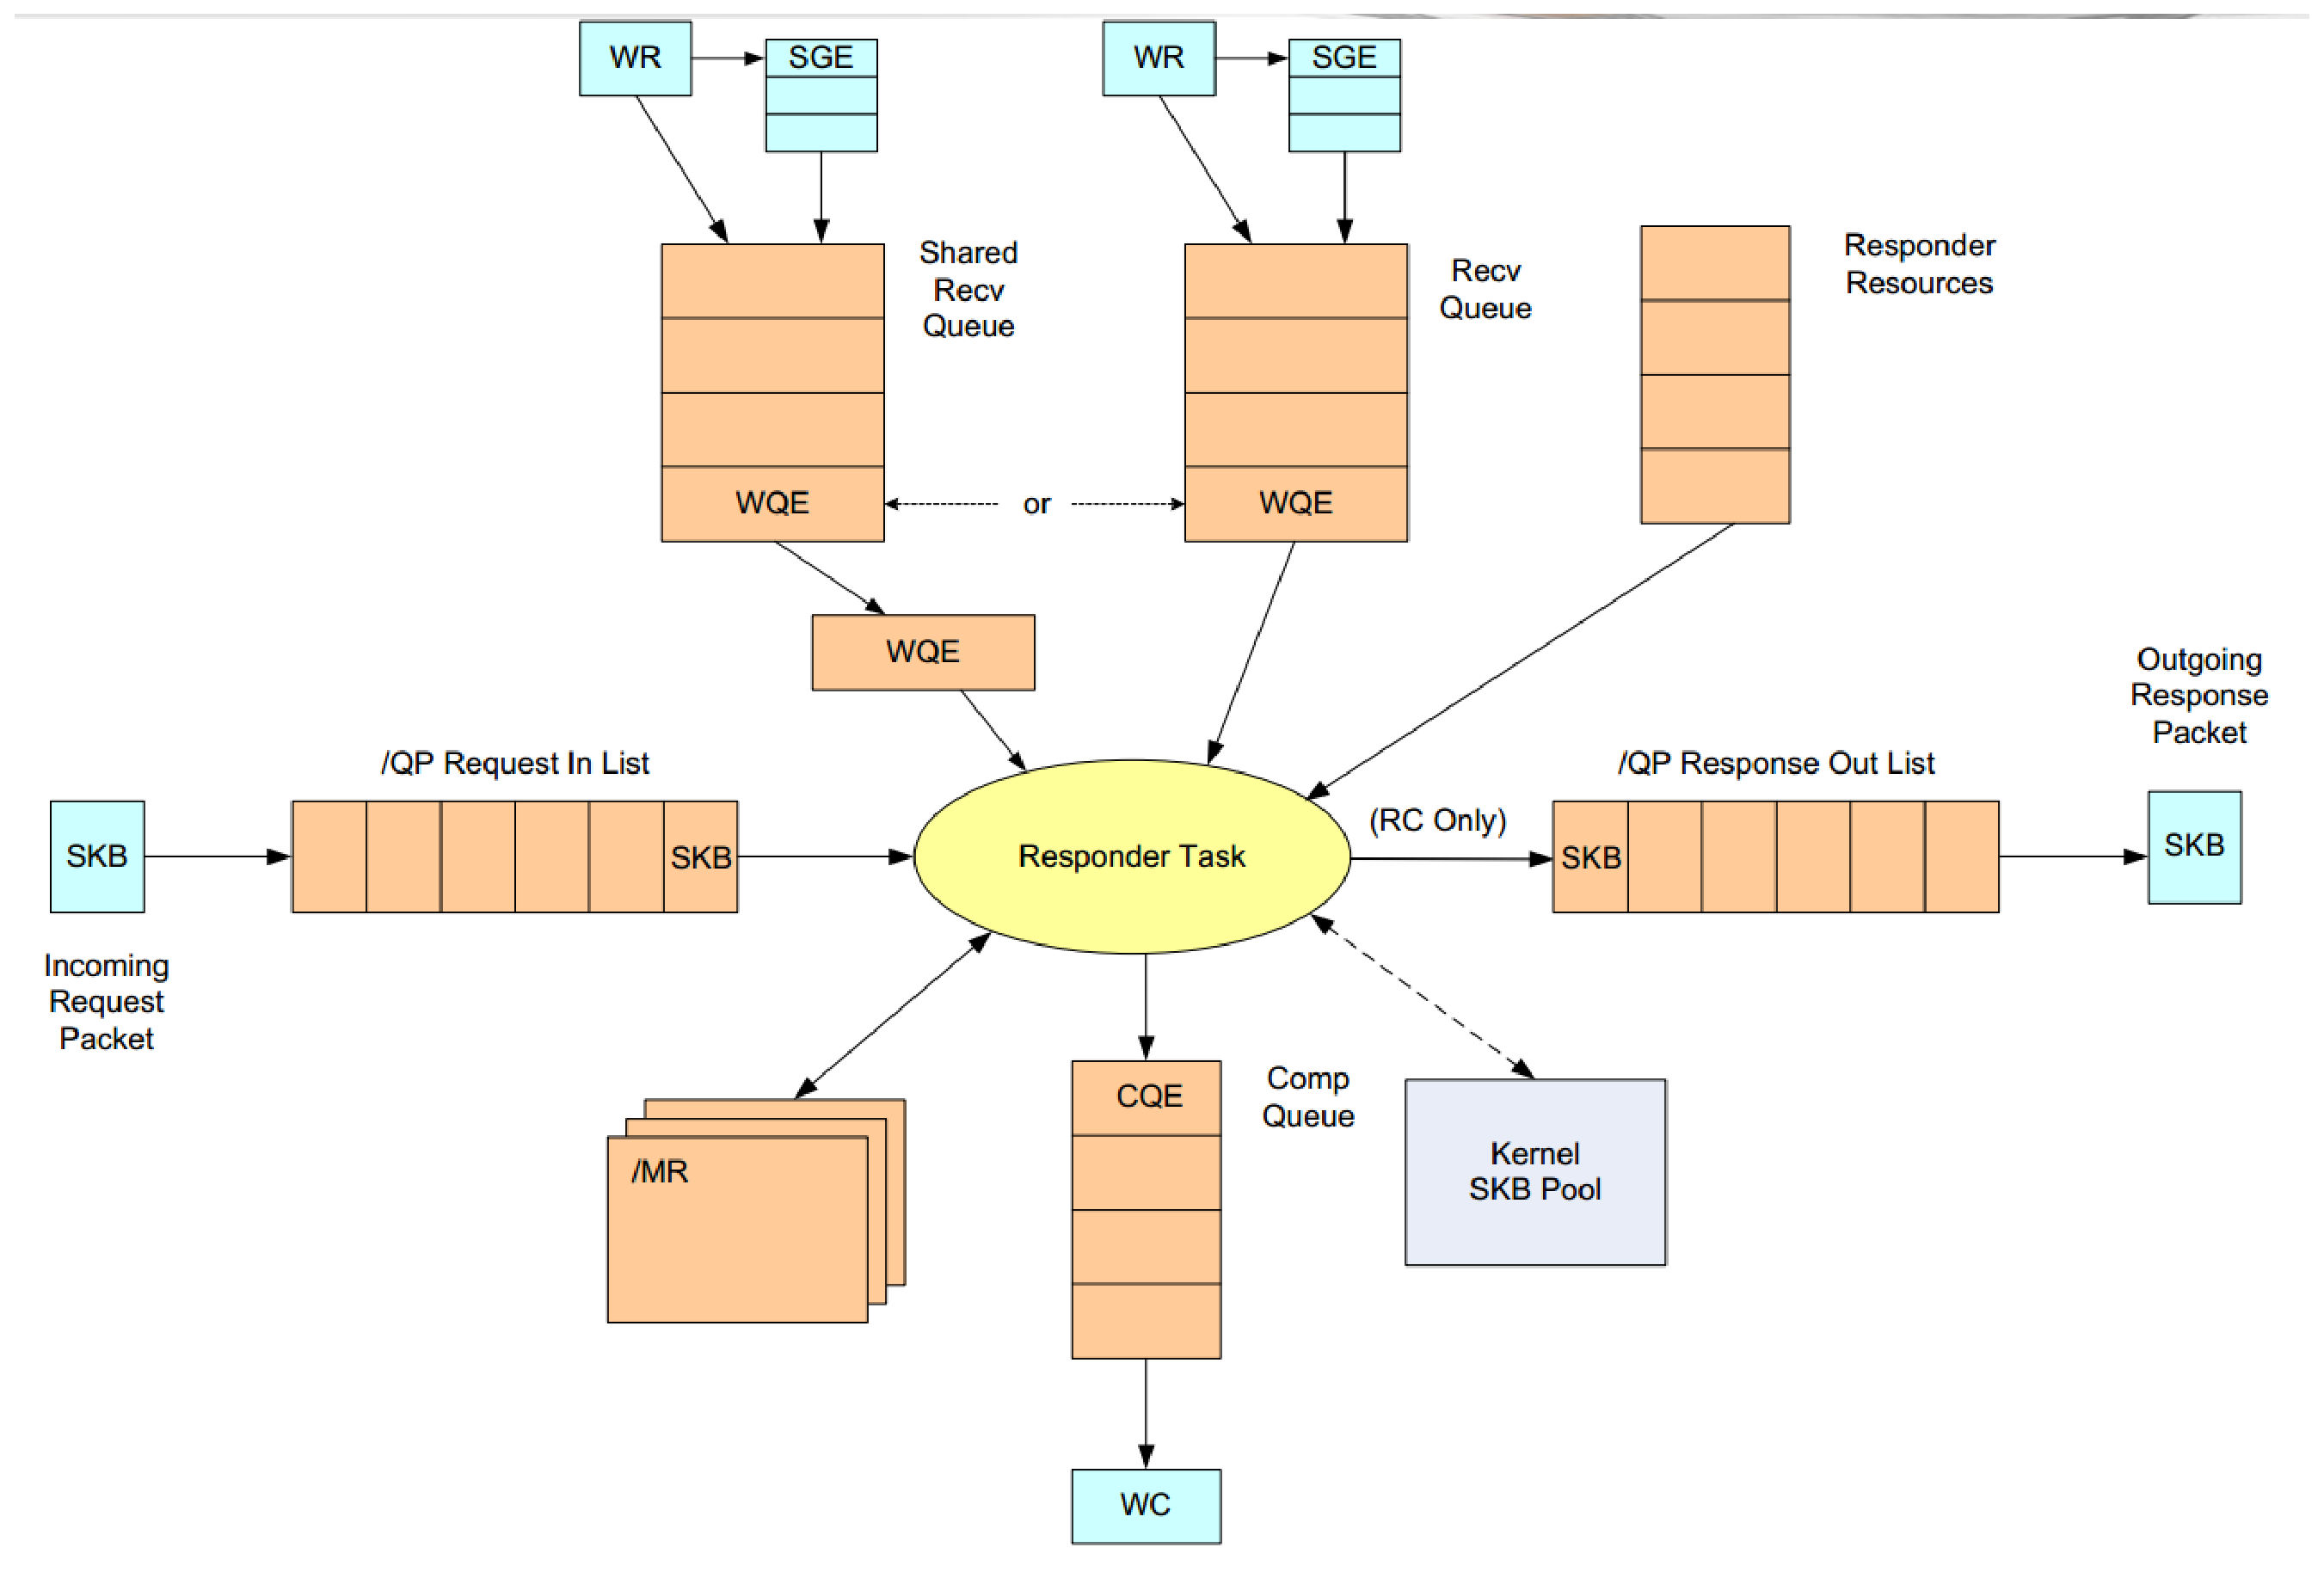
\includegraphics[width=\textwidth]{rxe_resp}
\caption{rxe QP Responder architecture \protect\cite{pearson-10}}
\label{rxe-resp}
\end{figure}

The QP Responder's architecture is illustrated in \textbf{Figure
  \ref{rxe-resp}}. The Responder partition contains functions that respond to
incoming requests for data. Such a request can be in one of two forms: a socket
buffer (SKB) sent from \verb;rxe-net; or a WR from a receive queue. In either
case, the Responder retrieves the requested data and generates a CQE
\cite{pearson-10}. If the connection associated with the request uses Reliable
Connection (RC) semantics, then a response message is generated and placed in
the send queue \cite{InfiniBandTARoCE-10}\cite{pearson-10}. Additonally, if a
request represents an atomic operation, the responder must save some state in
order to support retries for all message semantics and unordered read/write
operations for RDMA semantics. In \textbf{Figure \ref{rxe-resp}}, this is
represented by the ``Responder Resources'' data structure.

\begin{figure}[H]
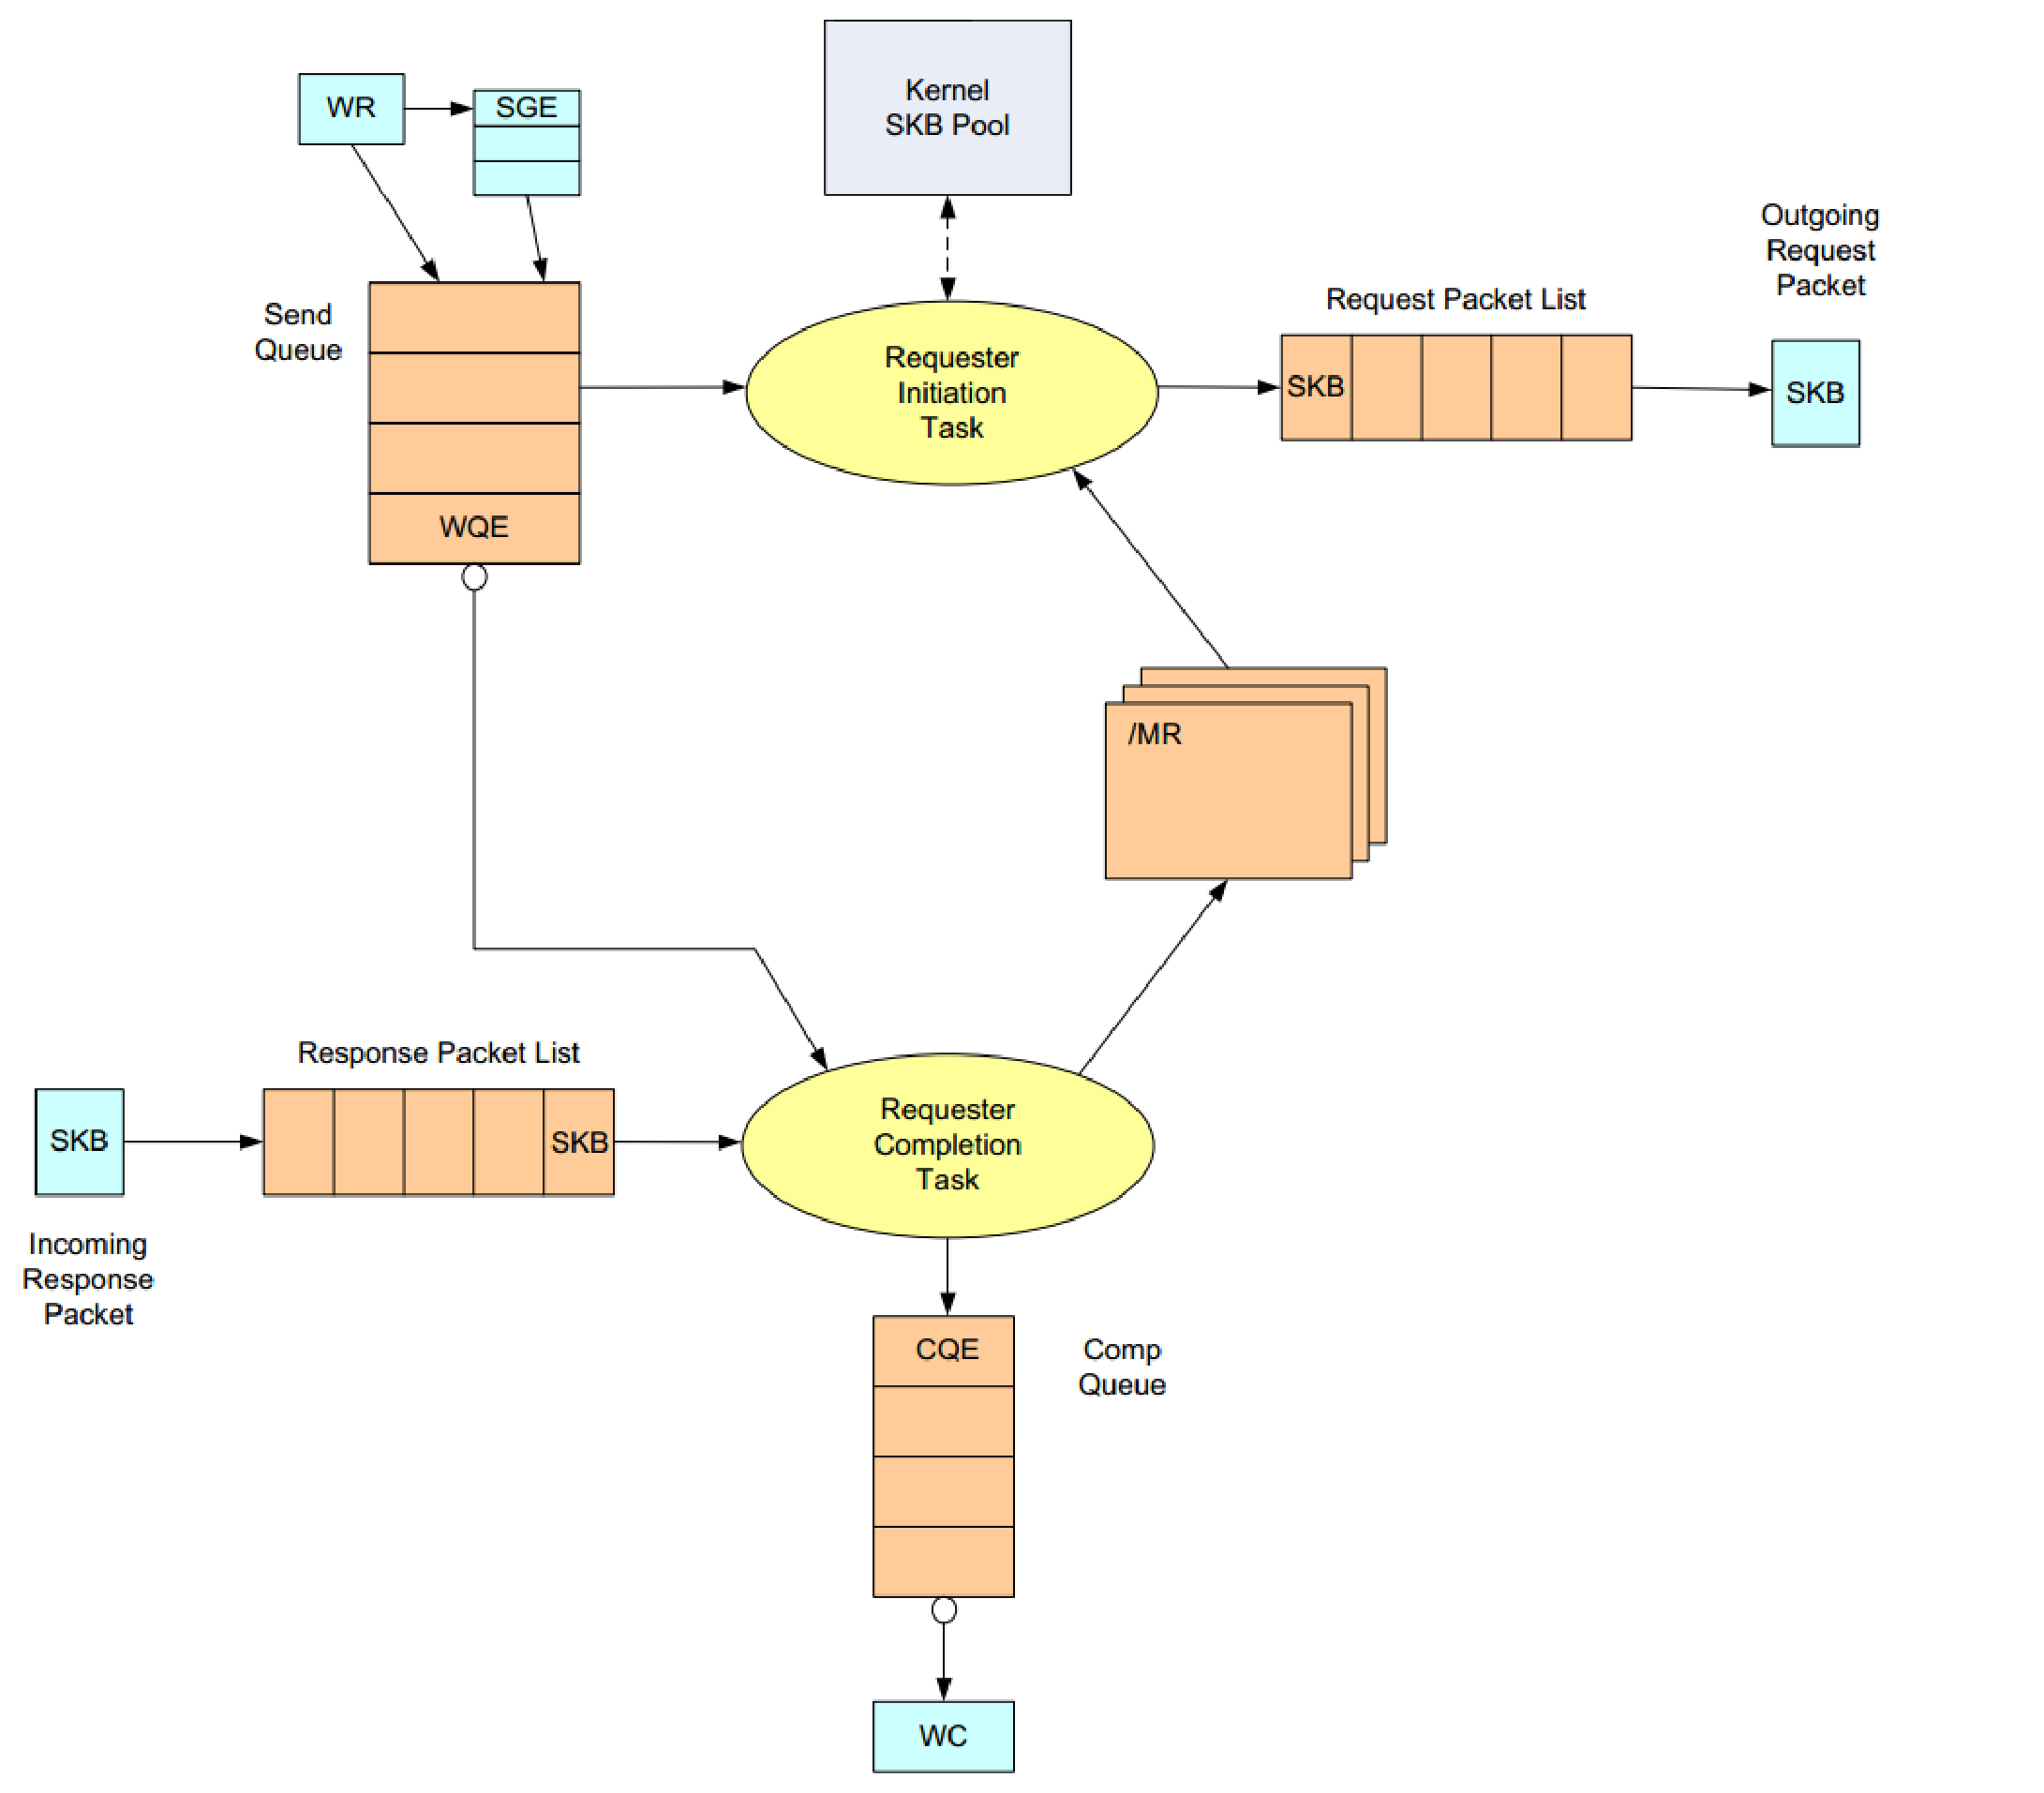
\includegraphics[width=\textwidth]{rxe_req}
\caption{rxe QP Requester architecure \protect\cite{pearson-10}}
\label{rxe-req}
\end{figure}

The QP Requester's architecture is illustrated in \textbf{Figure
  \ref{rxe-req}}. The Requester is further divided into an Initiator task and a
Completer task. The Initiator simply creates a request message for every entry
in the send queue. The Completer is active only for communication using the
Reliable Connection (RC) channel semantics. It waits for responses from the
remote node to indicate that each WQE has been retired\cite {pearson-10}. It
then generates a CQE and releases the WQE. If a message fails and must be
retried, the Initiator can be reset to the point where the Completer is
waiting. For all other channel sematics, the WQE is retired and released
immediately by the Initiator without invoking the Completer.

\begin{figure}[H]
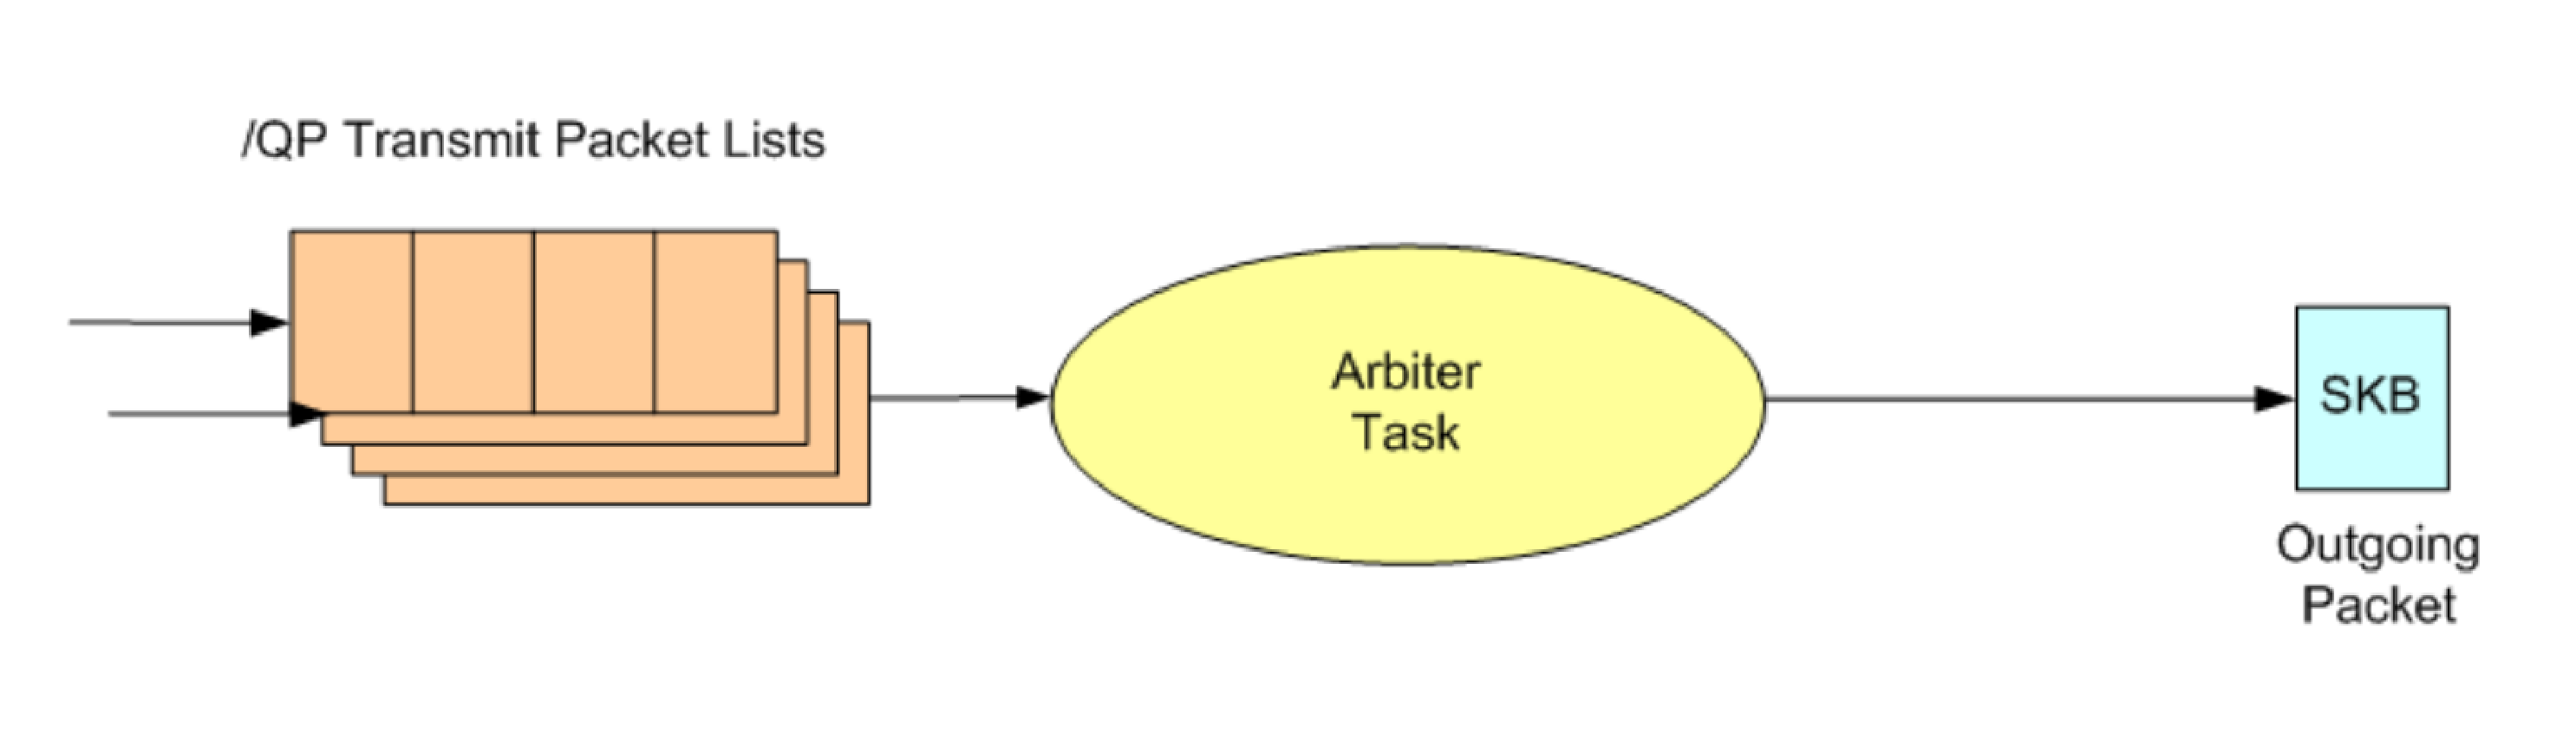
\includegraphics[width=\textwidth]{rxe_arbiter}
\caption{rxe Arbiter architecture \protect\cite{pearson-10}}
\label{rxe-arbiter}
\end{figure}

The Arbiter task is illustrated in \textbf{Figure \ref{rxe-arbiter}}. It
schedules actual transmission of outgoing messages. It implements a round-robin
scheduling policy among all active send queues, and it also handles flow control
in order to avoid packet dropping in Linux due to queue overrun
\cite{pearson-10}. This flow control includes a static minimum time between
packet transmissions. This parameter and others in the Arbiter can be tuned
while the module is loaded, and the Arbiter can even be disabled
altogether. In our research with the ODROID-U2, lowering or removing these
timing thresholds had no effect on end-to-end latency on a 100 Mbps Ethernet
link.

\subsection{\textbf{rxe-net}}

In many ways, the \verb;rxe-net; module functions as a wrapper for the
\verb;rxe; transport module described in \textbf{Section \ref{rxe}}. It
implements most of layer 3 of RoCE, allowing the layer 4 and higher functions of
\verb;rxe; to integrate with the existing layer 2 networking implementation in
Linux by forming a bridge that communicates with Linux on both the RDMA and
Ethernet sides. It can be envisioned as the horizontal portion of the \verb;rxe;
driver in \textbf{Figure \ref{rxe-linux}}. In addition to facilitating this
communication and marshalling of data, \verb;rxe-net; writes the appropriate
combination of Infiniband and MAC headers to each packet in order to fulfill the
requirements of the RoCE specification \cite{pearson-10}
\cite{InfiniBandTARoCE-10}. In accordance with the specification, the Ethernet
MAC (layer 2) header is identical to a normal ethernet packet except for the
ethertype value, which is set to \verb;0x8915; for all RoCE packets
\cite{InfiniBandTARoCE-10}. \textbf{Figure \ref{roce-packet}} compares normal
Infiniband packets to RoCE packets \cite{ayoub-11} \cite{InfiniBandTABase-07}
\cite{InfiniBandTARoCE-10}.

\begin{figure}[h]
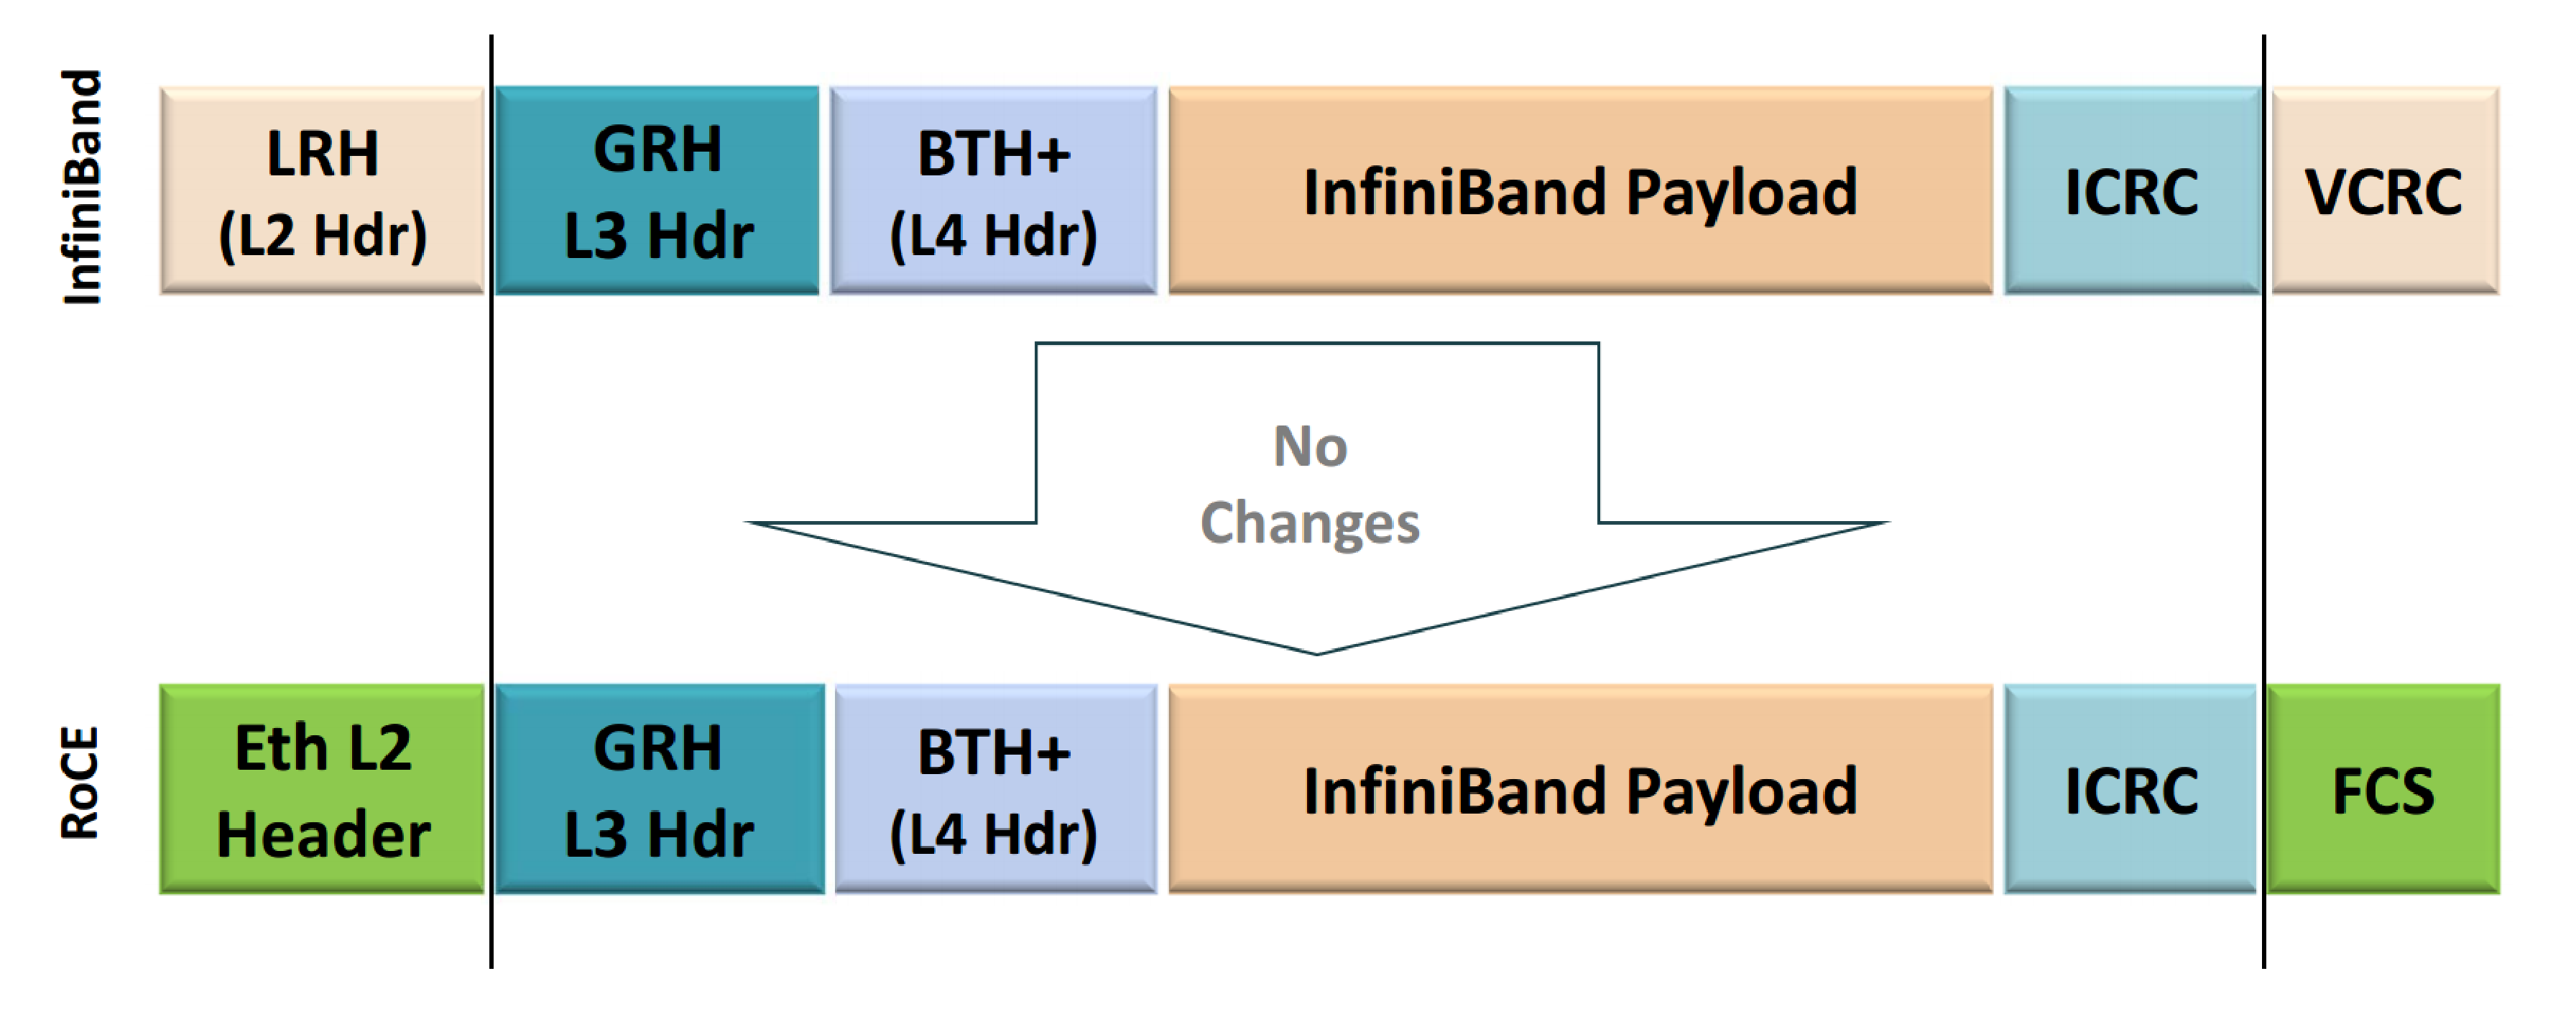
\includegraphics[width=\textwidth]{roce_packet}
\caption{RoCE packet composition \cite{ayoub-11}}
\label{roce-packet}
\end{figure}

\subsection{\textbf{Porting rxe to the ODROID Platform}}

%% TODO: Expand on this section a bunch. Include details of porting work

Although \verb;rxe; is designed to operate with any Ethernet adaptor, it also
depends on the IB libraries in the Linux kernel. These libraries, in turn,
depend on the presence of a PCI bus in the host system. Neither the ODROID-U2
nor the ODROID-XU has PCI support. Simply enabling PCI support in the Linux
kernel configuration creates some incompatibilites that must be resolved before
the kernel will work correctly. After some trial and error, I found an elegant
solution: the addition of the line in \textbf{Figure \ref{pci_code}} near the
beginning of \verb;drivers/pci/probe.c;.

\begin{figure}[h]
\centering
\begin{verbatim}
#define pcibios_assign_all_busses() 1
\end{verbatim}
\caption{Code added to drivers/pci/probe.c}
\label{pci_code}
\end{figure}

The most significant porting effort involved updating the \verb;rxe; driver to
work correctly with the ARM linux memory model. ARM Linux has several subtle
differences from x86 Linux in the way the kernel maps memory. This resulted in
some incompatibilities with the rxe code. Chiefly, the rxe code does not support
the mapping of high memory (userspace memory) into low memory (kernel memory) at
runtime. This is an important feature in modern IB drivers because it allows
memory regions to be directly accessed by userspace programs, eliminating some
need for high-latency context switches. \verb;rxe; currently uses the
\verb;page_address(); macro to get virtual page addresses. These calls should be
replaced by \verb;kmap(); or \verb;kmap_atomic(); in order to make them safe for
use on high memory pages. However, each \verb;kmap(); call requires a
corresponding \verb;kunmap();. Some of the \verb;rxe; DMA memory mapping
functions use the \verb;page_address(); macro to return an address for DMA
operations. This is not an intended use for \verb;kmap();, because the kernel
has a limited number of such mappings available. We were able to run the driver
recoded in this manner for use with micro-benchmarks, but it is unstable when
used with MPI applications. We concluded that a major overhaul of the \verb;rxe;
DMA architecture would be required to support high memory on the driver side.

Luckily, this problem is easily resolved by configuring the kernel to map all
memory to a single region, eliminating the distinction between user and kernel
address space. The ODROID-U2 and ODROID-XU only have 2046 MB of main memory, so
a 32-bit processor can map it all into a single address space. However, the
\verb;vmalloc; virtual memory region can overlap with some of this space,
causing the Linux kernel to ignore or truncate regions of address space that
should be mapped to physical memory. This limitation can be partially bypassed
by reconfiguring the size of the \verb;vmalloc; region using Linux kernel
parameters \cite{vmalloc-overlap}. Additionally, it is possible to move the
region by altering the values of the \verb;VMALLOC_START; and \verb;VMALLOC_END;
macros, then shifting the \verb;IO_ADDRESS; macro accordingly so memory-mapped
I/O devices still have their own address space. For the ODROID-XU, this process
enabled the use of 1884 MB of memory, while the remaining 163 MB were dedicated
to I/O devices. The final address space mapping is shown in \textbf{Figure
  \ref{addrmap}}.

The migration from the ODROID-U2 to the ODROID-XU presented some additional
challenges in the porting effort for the rxe driver. I encountered a bug that
disrupted the marshalling of Work Requests from userspace to kernel space. This
bug was a symptom of TODO. This problem can be solved by TODO.

\begin{figure}[h]
\begin{center}
\begin{verbatim}
Memory: 2046MB = 2046MB total
Memory: 1927936k/1927936k available, 167168k reserved, 0K highmem
Virtual kernel memory layout:
    vector  : 0xffff0000 - 0xffff1000   (   4 kB)
    fixmap  : 0xfff00000 - 0xfffe0000   ( 896 kB)
    vmalloc : 0xc0000000 - 0xff000000   (1008 MB)
    lowmem  : 0x40000000 - 0xbfe00000   (2046 MB)
    modules : 0x3f000000 - 0x40000000   (  16 MB)
      .text : 0x40008000 - 0x409ce000   (10008 kB)
      .init : 0x409ce000 - 0x40a0dfc0   ( 256 kB)
      .data : 0x40a0e000 - 0x40ab8a98   ( 683 kB)
       .bss : 0x40ab8abc - 0x40c7d758   (1812 kB)
\end{verbatim}
\end{center}
\caption{Address space mapped by Linux kernel}
\label{addrmap}
\end{figure}

\section{\textbf{Polling the Network Adaptor}}

Previous research with network drivers has shown that interrupt latency in a
multi-tasking operating system can be eliminated with a polling network driver
\cite{dovrolis-01}\cite{liu-09}. In fact, the Linux TCP/IP networking stack has
moved to a hybrid of polling and interrupt-based event processing that is
intended to reduce average network latency in high-traffic situations. In
Parallel Discrete Event Simulation on multi-core processors, it is often
advantageous to give up a processor core to a polling driver in order to
significantly reduce message latency for all packets. The big.LITTLE processor
configurations in products like the ODROID-XU make this prospect especially
enticing when one considers that polling could be handled by one of the
``little'' cores, leaving all the ``big'' cores available for event processing.

Although the ability to symetrically multi-process with both ``big'' and
``little'' cores is not yet present for Linux in the ODROID-XU, we pursued this
goal in the hope that the trade of a ``big'' core for reduced latency would
still be worthwhile. Doug Weber and Zakaria Aldeneh began this study by creating
an EHCI polling driver for use with the standard ODROID-XU network
adaptors. Weber and I later extended this work to an XHCI polling driver used
with the Gigabit Ethernet adaptors for the ODROID-XU.

\subsection{\textbf{EHCI Polling Driver}}

%% TODO: Get info from Doug

\subsection{\textbf{XHCI Polling Driver}}

%% TODO: Get info from Doug

\newpage
\chapter{Cluster Implementation and Testing}
\label{cluster}

Three primary testing platforms were used for the experiments presented in this
thesis.

\section{\textbf{Two ODROID-U2 Nodes}}

Preliminary work with RoCE was tested on two ODROID-U2 computers running Debian
7.0-armhf with Linux kernel 3.0.90. The ODROID-U2 nodes are connected to an
unmanaged Gigabit switch through Category 6 Ethernet cables. Unless specified
otherwise, the Linux network MTU is set to 1488 bytes and the RoCE MTU is set to
1024 bytes.

\section{\textbf{Two ODROID-XU Nodes}}

Doug Weber and Zakaria Aldeneh performed their initial work with EHCI polling on
two ODROID-XU nodes running the Linux kernel 3.4 connected to an unmanaged
Gigabit Ethernet switch using the nodes' 100 Megabit ethernet adaptors.
%% TODO: Get more info from Doug

\section{\textbf{Final Cluster}}

The success of RoCE and EHCI polling experiments motivated the purchase of two
additional ODROID-XU nodes as well as Gigabit Ethernet adaptors for all four
nodes.
%% TODO: Get two nodes from Doug
%% TODO: set up cluster

\newpage
\chapter{Results}
\label{results}

\section{\textbf{Micro-benchmark Results}}

Preliminary micro-benchmark results from a cluster of two ODROID-U2 nodes are
presented first. Next, the results of similar tests on the four-node ODROID-XU
cluster are shown.

\subsection{\textbf{Two ODROID-U2 Nodes}}

Figures \ref{npmpi-llat} and \ref{npmpi-hlat} show MPI message latency for small
messages and large messages, respectively. Latency over RoCE is 17\% to 31\%
lower than latency over TCP for messages smaller than 260 B. In fact, RoCE
latency remains flat throughout that region, while TCP performance degrades
slowly as message size increases. This trend of identical performance for all
messages from 0 to around 256 B continues throughout this section. We believe
that this is a manifestation of a performance limitation introduced by the
USB-to-Ethernet translation in the LAN9730 hardware.
%% TODO: We will discuss this further in Section \ref{discussion}.

\begin{figure}[H]
\includegraphics[width=\textwidth]{netpipe_lat_small}
\caption{NetPIPE MPI Latency Results, Small Message Sizes}
\label{npmpi-llat}
\end{figure}

The trend of performance improvement with RoCE continues until message size
rises above 8 KB, after which RoCE latency is significantly higher than TCP
latency. %% This was actually really surprising. Can't explain it...yet

\begin{figure}[H]
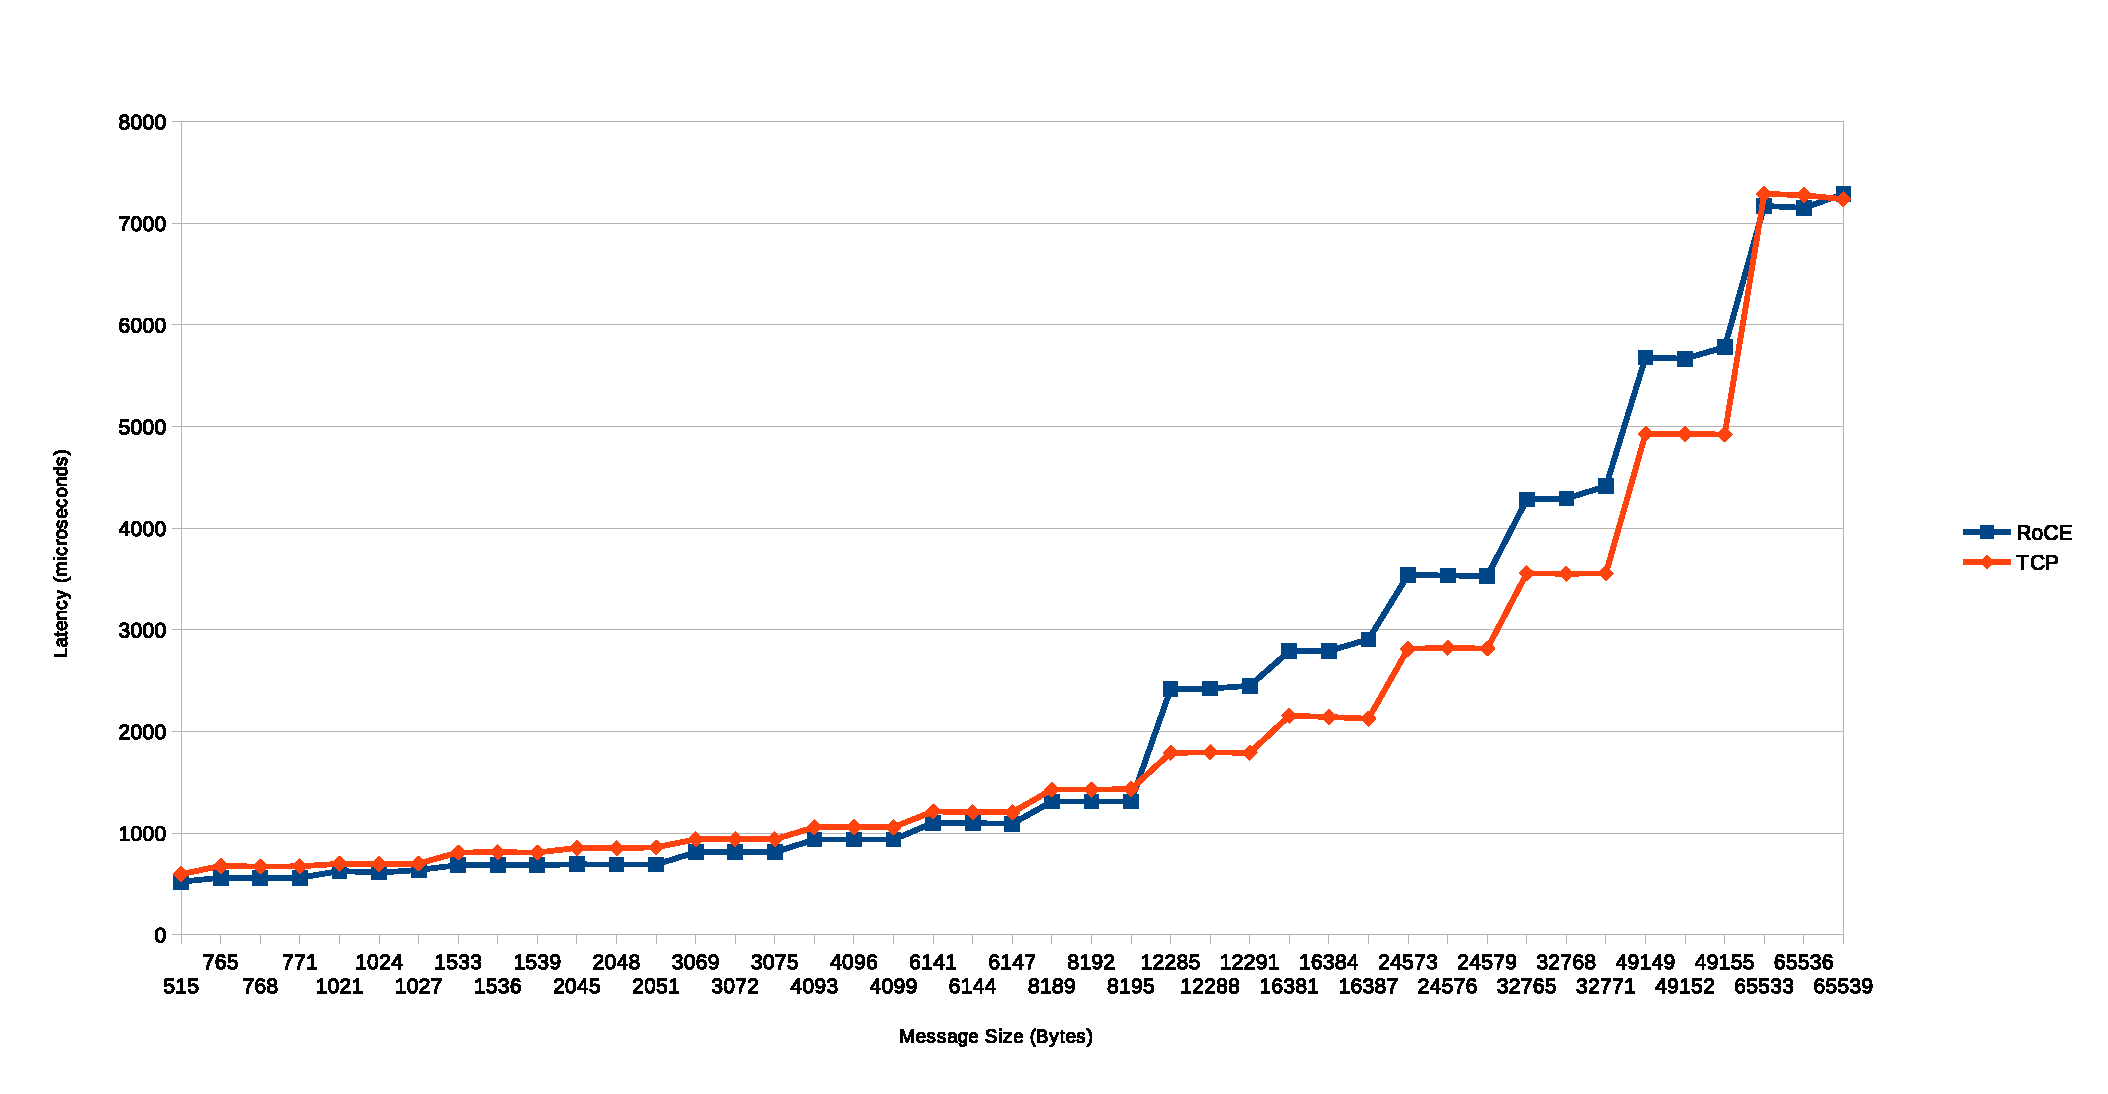
\includegraphics[width=\textwidth]{netpipe_lat_large}
\caption{NetPIPE MPI Latency Results, Large Message Sizes}
\label{npmpi-hlat}
\end{figure}

The MPI bandwidth results in Figures \ref{npmpi-lbw} and \ref{npmpi-hbw} mirror
the latency results. Interestingly, neither TCP nor RoCE traffic could saturate
the 100 Mbps link. %% Is this because the processor can't move data around
%% fast enough? If so, this could have implications on the discussion of GbE
%% modules for the XU. We could also blame the NIC, Linux, or even NetPIPE. I
%% might have to add a way to bypass the \verb;rxe; flow control...

\begin{figure}[H]
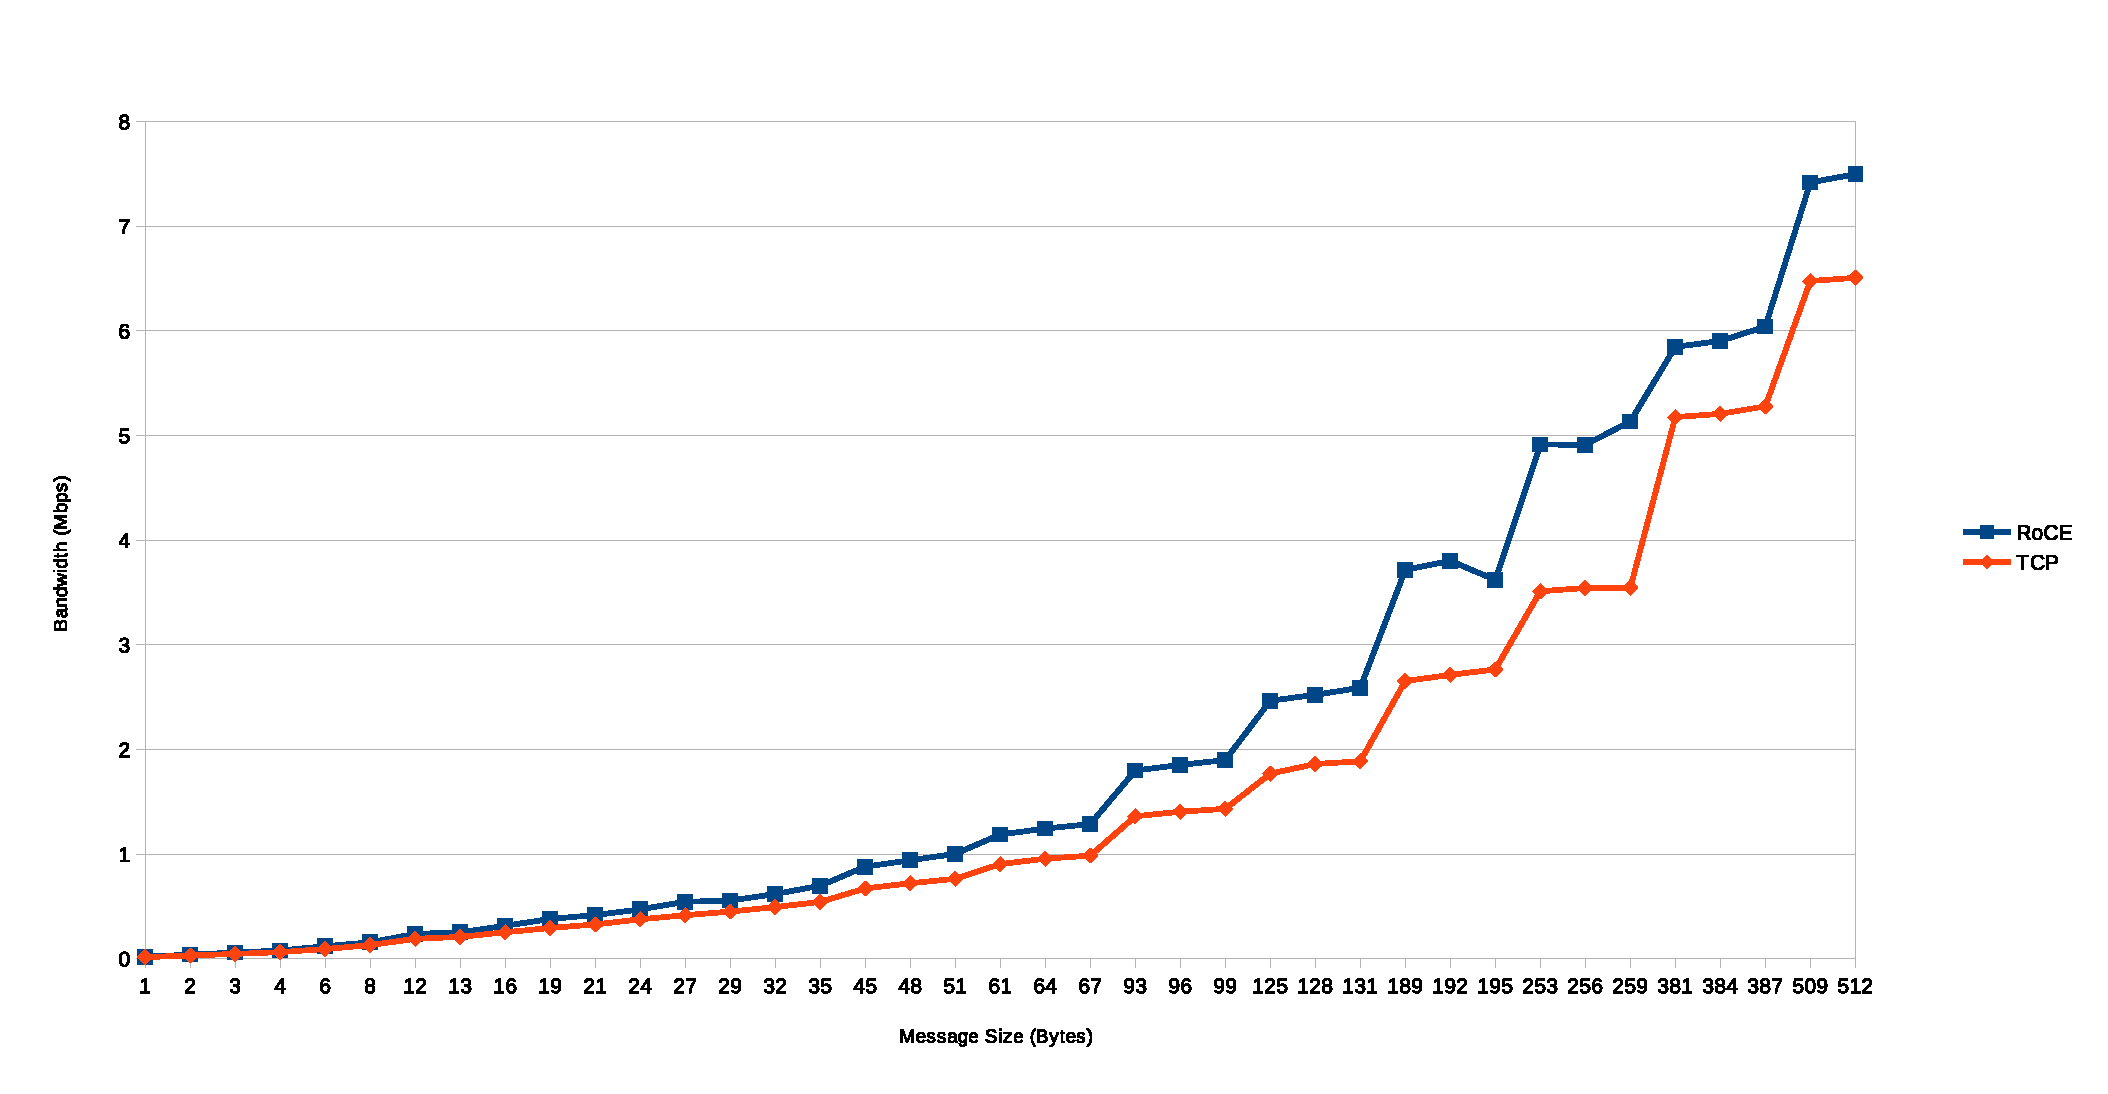
\includegraphics[width=\textwidth]{netpipe_bw_small}
\caption{NetPIPE MPI Bandwidth Results, Small Message Sizes}
\label{npmpi-lbw}
\end{figure}



\begin{figure}[H]
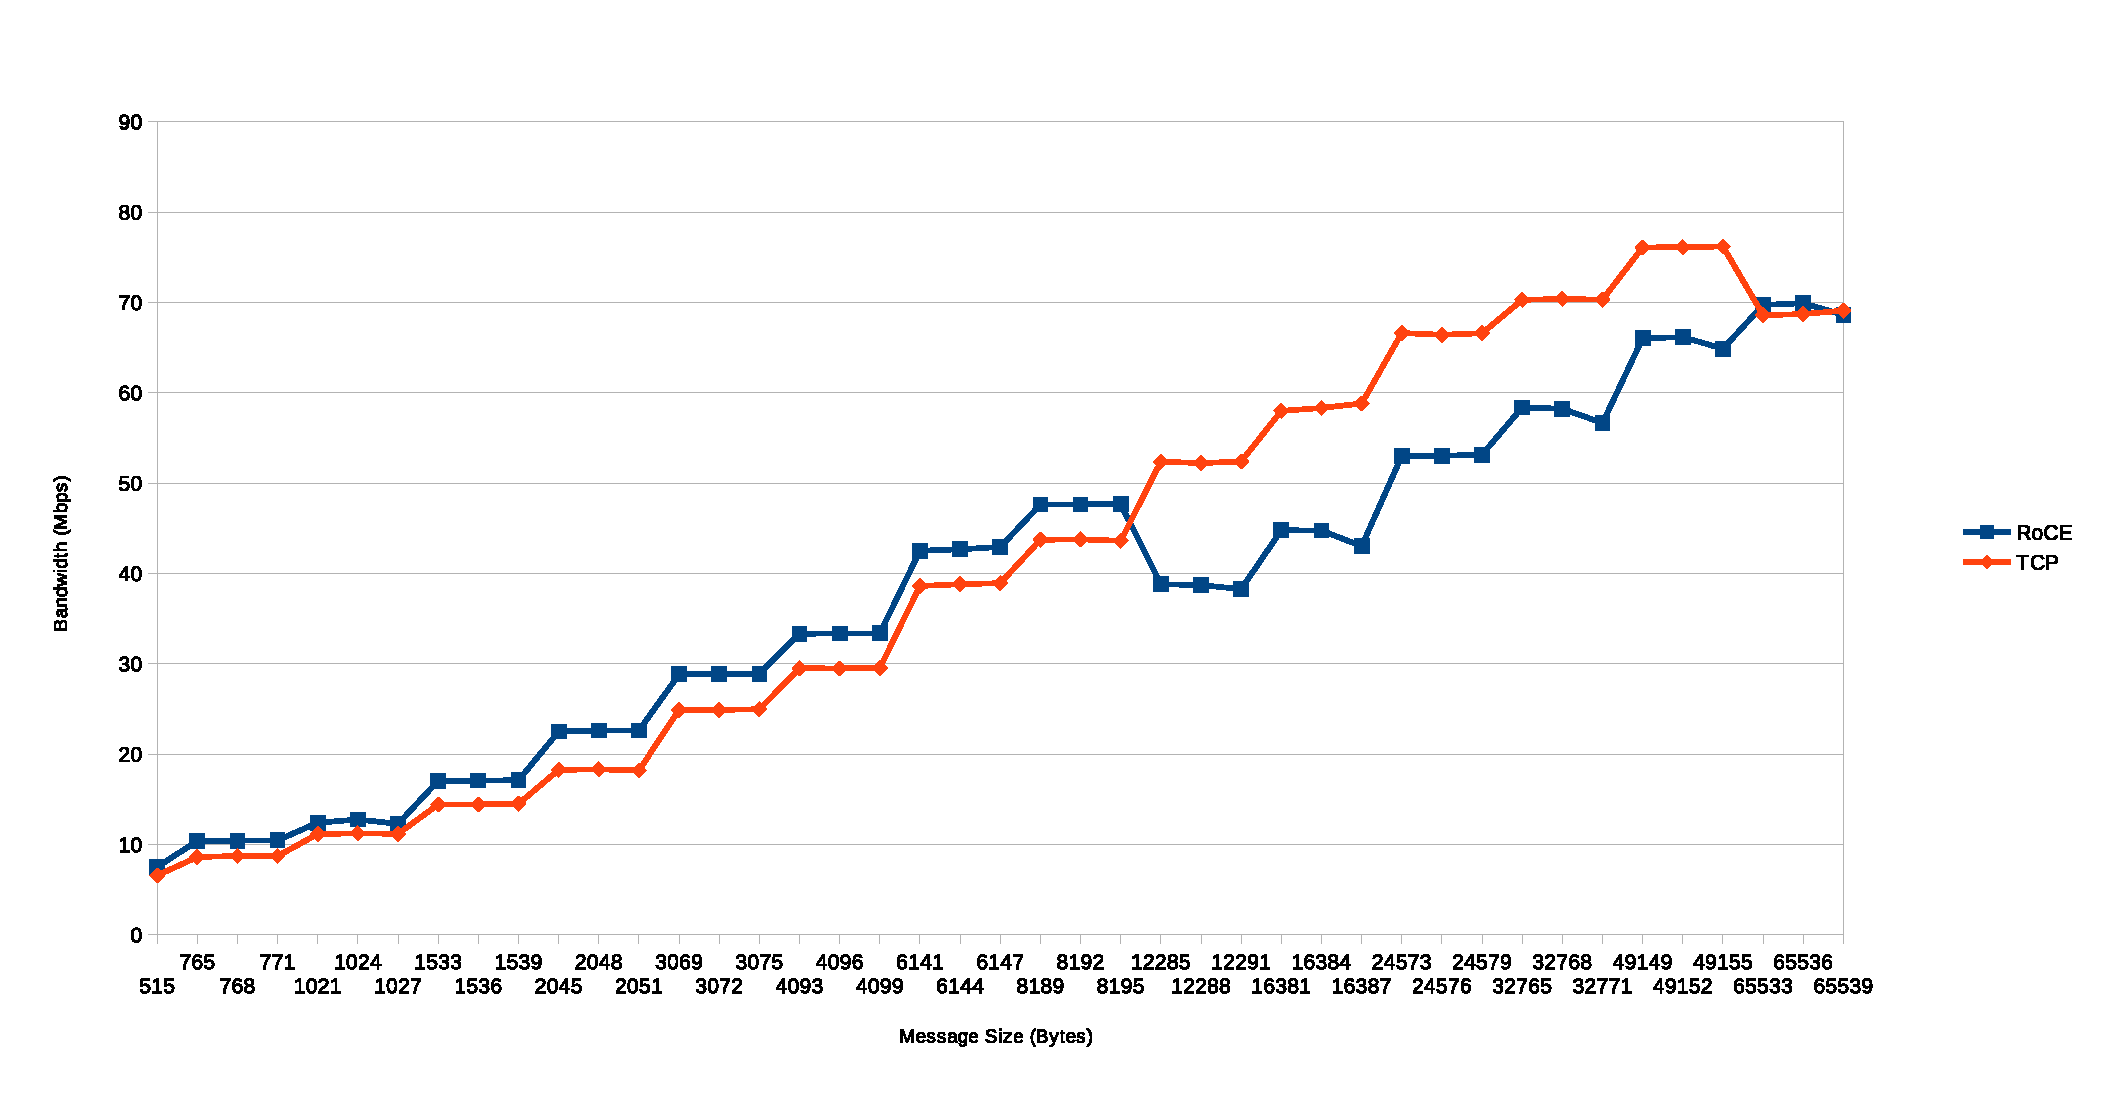
\includegraphics[width=\textwidth]{netpipe_bw_large}
\caption{NetPIPE MPI Bandwidth Results, Large Message Sizes}
\label{npmpi-hbw}
\end{figure}

In order to test transport scalability over MPI in the ODROID platform, we used
the Intel MPI Benchmarks (IMB) suite's ``MultiPingPong'' test with four, six,
and eight MPI processes. This benchmark creates pairs of processes that perform
a standard ping-pong test in parallel with the other pairs. We suspected that
the reduced CPU requirements of the IB transport would lead to slower scaling of
latency as network and I/O bus congestion increases. Figure \ref{multipingpong}
supports this conjecture. In fact, the \verb;rxe; driver appears to thrive in a
congested networking environment, while TCP/IP latency grows steadily. It
appears that the increased network activity may be hiding some of the latency
introduced by the Ethernet adaptor. %% TODO: How?

\begin{figure}[H]
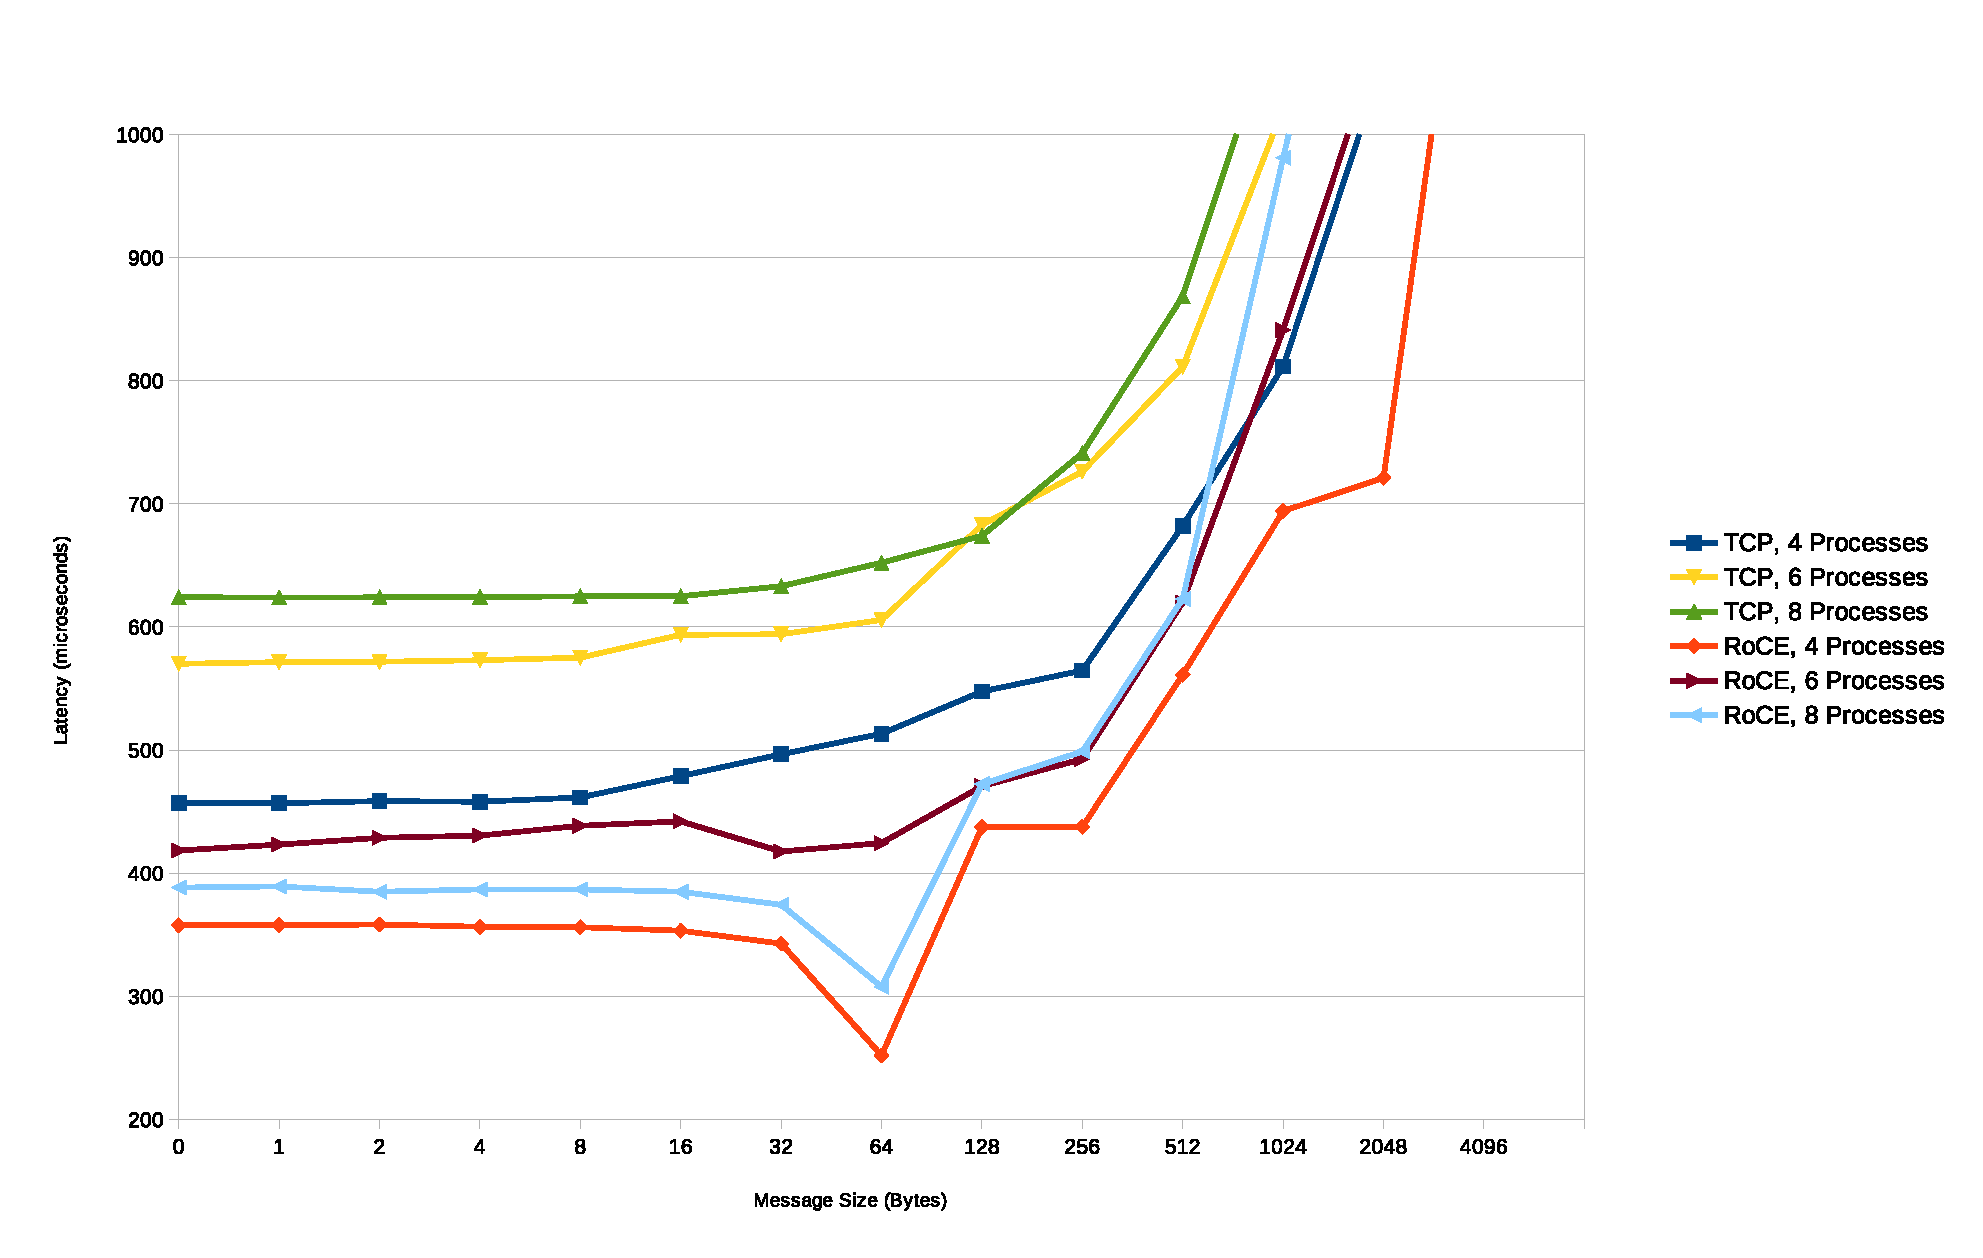
\includegraphics[width=\textwidth]{pingpong_multi_zoom}
\caption{Scaling of Message Latency with Link Congestion}
\label{multipingpong}
\end{figure}

\subsection{\textbf{Final Cluster}}

\section{\textbf{Parallel Discrete Event Simulation Results}}

\href{https://github.com/carothersc/ROSS}{Rensselaer's Optimistic Simulation
  System (ROSS)} is used for all PDES experiments. It uses MPI for all
inter-process communication, including local communication \cite{carothers-02}.

\newpage
\chapter{Conclusions}
\label{conclusions}

\newpage
\bibliographystyle{abbrv} \bibliography{refs}

\end{document}
